\chapter{Radio Antennas and Interferometry}\label{Chapter2}  % Main chapter title

% For referencing the chapter elsewhere, use \ref{Chapter1} 
% ------------------------------------------------------------------------------------------------------------------------------
% Define some commands to keep the formatting separated from the content 
% \newcommand{\keyword}[1]{\textbf{#1}}
% \newcommand{\tabhead}[1]{\textbf{#1}}
% \newcommand{\code}[1]{\texttt{#1}}
% \newcommand{\file}[1]{\texttt{\bfseries#1}}
% \newcommand{\option}[1]{\texttt{\itshape#1}}

%\lhead{Chapter 2. \emph{Radio Telescope Antennas \& Super-Synthesis Technique}}

% --------------------------------------------------------------------------------------------------------------------------------
\textbf{Overview}\\
% \HRule \\[0.4cm]
\par\noindent\rule{\textwidth}{0.4pt}\\
\textit{Chapter Two introduces us to the general antenna parameters that are significant to describing the operation and performance of an antenna. A further
discussion is made on how to mathematically derive the Stokes parameters from wave propagation. Types of radio arrays are also discussed in this section. 
Finally, a brief description of radio interferometry is given.}
\par\noindent\rule{\textwidth}{0.4pt}\\
% \HRule \\[1.5cm]
% -------------------------------------------------------------------------------------------------------------------------------------


\section{Introduction}	  \label{chap2:sec1}
%
\theo{
The fundamental laws that govern the complete EM  phenomena  can be explained by the famous Maxwell’s equations as follows: \\
%%
%%
\begin{itemize}
 \item The Gauss' law for electric field is defined as: 
 %%
 \begin{equation} \label{eq:gauss_theorem1}
 \oint \vec{\xi}. \vec{ds} = \frac{q}{\epsilon_0}
 \end{equation} 
 %%
 where the charge $q$ is circumscribed within a closed region and $\epsilon_{0}$ is electric constant (also known as electric 
permittivity of free space).   This relation means that whenever there is a charge $q$, there exist
 an electric field $\vec{\xi}$ and of course, anytime there is $\vec{\xi}$, there exist $q$.
 %% 
 \item The Gauss' law for magnetic field is defined as: 
 %%
 \begin{equation} \label{eq:gauss_theorem2}
 \oint \vec{\mathcal{B}}. \vec{ds} = 0
 \end{equation} 
 %%
 This equation shows that a magnetic field $\vec{\mathcal{B}}$ is always defined in a closed line. Here, $\vec{\mathcal{B}}$ has no 
 static point and no termination.
 %%
 \item Equation~\ref{eq:Faraday} is Faraday's law  of EM induction:
 %%
 \begin{equation} \label{eq:Faraday}
V_{k} = - \frac{d\phi_{\mathcal{B}}}{dt}  
 \end{equation}
%%
Here, the rate of change of magnetic flux is equal to the voltage induced $V_{k}$ and therefore, this induced potential difference can be expressed
as $\oint \vec{\xi}. \vec{dr} = - \frac{d}{dt} \vec{\mathcal{B}}.A$ with $A$ being the cross section area. Note that whenever there is a change in 
$\vec{\mathcal{B}}$, we obtain $\vec{\xi}$.
%%
\item The fourth equation is Ampere-Maxwell's  law and this is given as:
 %%
 \begin{equation} \label{eq:amperes}
  \oint \vec{\mathcal{B}}. \vec{dl} = \mu_{0}i_{c} + \mu_{0}\epsilon_{0}\frac{d\phi_{\xi}}{dt}  
 \end{equation}
 %%
 where $\phi_{\xi}$ is the change in electric flux, $\vec{dl}$ is the direction of the current, $i_{c}$ is the conduction current and the magnetic constant (also known as magnetic permeability of free space) is denoted $\mu_{0}$. Equation~\ref{eq:amperes} shows that, a change in an electric field creates a magnetic field.
 %%
%%
\end{itemize}
} % @@@@@@@@@@@@@@@@@@@@@@@@@@@
% 
% % Q1 
% \begin{eqnarray}
%  \begin{aligned}
%   \left\{\begin{array}{r}
%                 \triangledown \times \bm{\varepsilon}(\bm{r},t) = -\frac{\partial }{\partial t}\bm{\mathcal{B}}(\bm{r},t) - \bm{\mathcal{M}}(\bm{r},t)\\
%                    \\
%                   \triangledown \times \bm{H}(\bm{r},t) = \frac{\partial }{\partial t}\bm{\mathcal{D}}(\bm{r},t) + \bm{\mathcal{J}}(\bm{r},t)
%                    \end{array}\right.
%                    \end{aligned}
% %   \phantom{\hspace{1cm}}
%   \label{eq:Maxwell_eqxn}
% \end{eqnarray}
% % 
% where,
% 
% \noindent $\bm{\varepsilon}(\bm{r},t)$ \quad electric field \quad $V/m$,\\
% $\bm{H}(\bm{r},t)$ \quad magnetic field  \quad $A/m$,\\
% $\bm{D}(\bm{r},t)$ \quad electric induction \quad $C/m^2$,\\
% $\bm{B}(\bm{r},t)$ \quad magnetic induction \quad $Wb/m^2$,\\
% $\bm{\mathcal{J}}(\bm{r},t)$ \quad electric current density (source) \quad $A/m^2$,\\
% $\bm{\mathcal{M}}(\bm{r},t)$ \quad magnetic current density (source)  \quad $V/m^2$.
%%
\theo{
\noindent The mathematical models in these four equations give a complete characterisation  of how the fields $\vec{\xi}$ and $\vec{\mathcal{B}}$ are produced and altered by each other. The term $\oint \vec{\mathcal{B}}. \vec{dl} = \mu_{0}\epsilon_{0}\frac{d\phi_{\xi}}{dt}$  in Equation~\ref{eq:amperes} depicts the existence of wave such that, $1/\sqrt{\mu_{0} \epsilon_0}$ gives the speed of the wave. Therefore, Equations~\ref{eq:Faraday} and~\ref{eq:amperes} are responsible for the prediction of 
EM wave due to the spatial and time variations of the fields. A  comprehensive understanding of Maxwell's equations can be obtained from \citep{hampshire2018derivation,fleisch2008student}.
} % @@@@@@@@@@@@@@@@@@@@@@@@@@@

\theo{In radio astronomy, we can intercept the EM wave with a \emph{radio telescope}. The instrument operates in a reception mode such that the electric current induced on the input terminals, converts into a radio frequency (RF) signal and we can observe the signal at different ranges, called \textit{bands}. 
Next, we present on the parameters of an antenna.} % @@@@@@@@@@@@@@@@@@@@@@@@@@@
% as presented in Table~\ref{table:1} according to the Institute of Electrical and Electronics Engineers (IEEE) standard. The KAT-7 can
% observe at L-band frequency which is very good for investigating HI IM experiments.

%
\section{Antenna Parameters} \label{chap2:sec2}
%
% \vspace*{-2em}
\theo{
The antennas we use in radio astronomy are devices that receive radio waves from the free
space and convert them into electrical signals. Numerous designs of an antenna make
it necessary to define how the instrument operates. This requires a clear understanding of
the parameters of the antenna and therefore, in this section, we present a review of some fundamental
parameters of an antenna discussed by \cite{Balanis2005}. 
} % @@@@@@@@@@@@@@@@@@@@@@@@@@@
% -------------------------------------------------------------------------------------------------------------------------------------

%
\subsection{Antenna Field Regions}	   \label{chap2:fzones}
%
\theo{
The antenna field zones illustrate how antenna radiates with respect to its position. There are basically three main classes of field zones 
as depicted in Fig.~\ref{fig:amp-pattern} and briefly discussed below:
  %
\begin{itemize}
 \item \textit{Reactive near-field}: It is the immediate region surrounding the antenna where electric and magnetic fields are mostly not in phase. The energy in this region usually turns back
 to the antenna in a regenerative manner (thus, there is back and forth oscillation of energy) hence, storing the energy is this region \citep{8251376}.
% 
%  The energy in this region oscillates towards and away from the antenna, making it purely reactive
%  and storing the energy completely. 
%  This makes both the electric and magnetic fields out of phase.
 The radius of this zone is computed as $r_1 < 0.62\left(\frac{D^3}{\lambda}\right)^{1/2}$, where $r$ is the separation
 from the antenna surface, $D$ is the size of the antenna and $\lambda$ is the wavelength in metres.
 The frequency of the EM wave is related to the wavelength such that, $\lambda = \frac{c}{\nu}$ where, $c \approx 3.0 \times 10^8 \,\mathrm{m/s} $ is the speed of light and $\nu$ 
 is the frequency in Hz. 
%  In Fig.~\ref{fig:amp-pattern}, we can clearly observe that there is no form of radiation in this field.
%
\item \textit{Radiating near-field} (also known as the \textit{Fresnel} region): It is the next region after the reactive near-field where the field distribution begins to have some 
regular pattern as displayed in  Fig.~\ref{fig:amp-pattern}. Thus, part of the energy obtained in this region converts into radiation. This is because in this zone, 
the EM fields are not directly in or out of phase hence, making the field strength to become less reactive as compared to the immediate field zone. 
The radius of this zone is determined as $r_2 < 0.62\,D^{2}/\lambda$.
%%
\item \textit{Far-field} (also known as the \textit{Fraunhofer} region): This region exists at a distance $r_3 > 2\,D^{2}/\lambda$. The reactive fields are no longer present and only the 
radiation fields exist. Here, the EM fields are directly orthogonal with constant amplitude. Furthermore, the 
general radiation pattern in this region remains the same regardless of the distance from the antenna. 
 \end{itemize}
%%
\noindent Therefore, as the space from the antenna changes from the near to the far fields, the radiation pattern of an antenna also varies in shape in terms of amplitude and phase.
In Fig.~\ref{fig:amp-pattern}, the radiation pattern is almost uniformly distributed in the reactive near-field region and gradually creates smooth lobes at the radiating near-field
and eventually, gets fully formed  at the far-field with minor and major lobes. In radio astronomy, the antenna of a radio telescope operates in the far-field of the feed system 
to produce the desired illumination of the antenna.
%%
  } % @@@@@@@@@@@@@@@@@@@@@@@@@@@
 % ++++++++++++++++++++++++++++++++++++++++++++++
% Fig. 2
% ++++++++++++++++++++++++++++++++++++++++++++++
%
%
\begin{figure}[H] %{\columnwidth}
	    \centering	
	    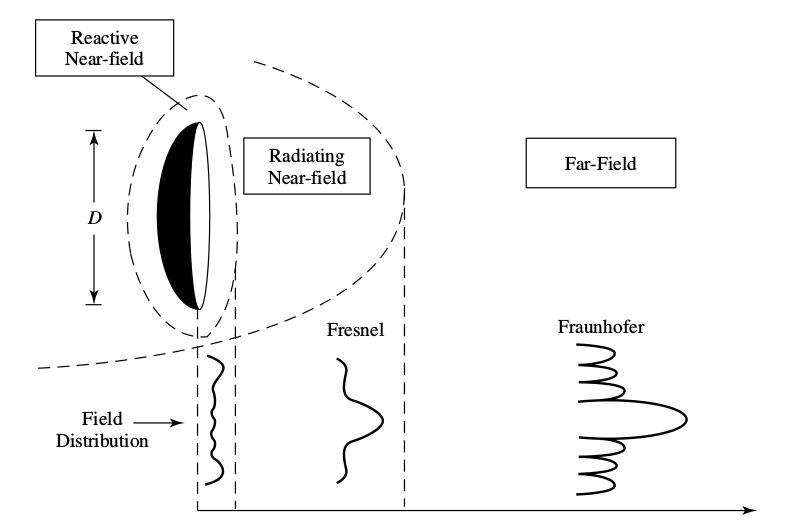
\includegraphics[width=12cm, height=9cm]{c2/amp-pattern}	   	   
	    \caption{An illustration of the various field distributions at each field zone. \emph{Source}: This figure  is reproduced from  \citep[pg. 35]{Balanis2005} 
	    but originally produced by \citep{482029}.}
	    \label{fig:amp-pattern}
       \end{figure}
  \FloatBarrier   
%%

% \begin{figure}[H]
% \centering
%  \begin{subfigure}{\columnwidth}     
%                 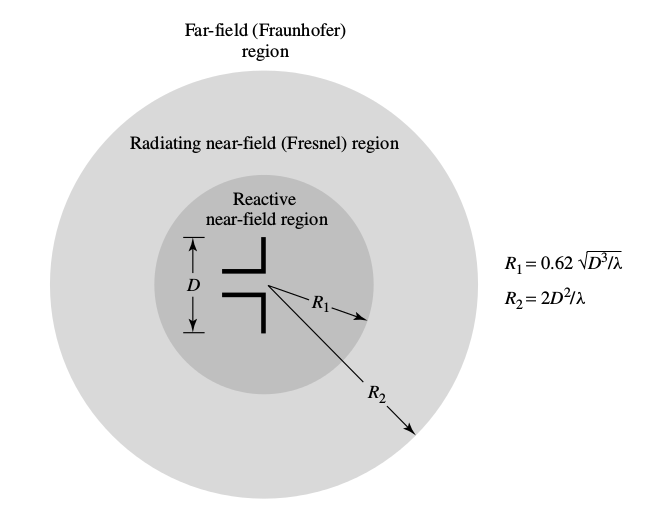
\includegraphics[width=\linewidth]{c2/field-regions2}               
%                 \caption{}                
%                 \label{fig:hg1}
%         \end{subfigure} 
%         %%
%         \begin{subfigure}{\columnwidth}
%                 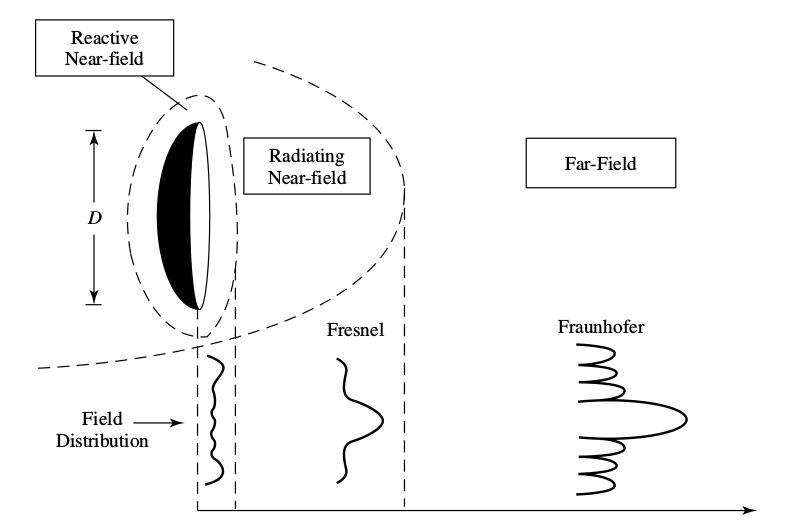
\includegraphics[width=\linewidth]{c2/amp-pattern}                
%                 \caption{}               
%                \label{fig:hg2}
%         \end{subfigure}        
%          \caption{The different field regions of an antenna. Source: This figure  is reproduced from  \citep[p. 34]{Balanis2005}.}%          
%          \label{fig:hgg}
%   \end{figure}
% \FloatBarrier


%
\subsection{Radiation Patterns}	   \label{chap2:RadiationPattern}
%
It is a visual description of the radiation properties of the antenna. The pattern of the antenna is mostly in 3D and measured in steradians, but 
can also be projected in a linear scale as shown in Fig.~\ref{fig:radiation-pattern}.  There are actually two main types of this pattern, namely:
%%
 \begin{itemize}[noitemsep]
  \item \emph{Field pattern}:- This is the amplitude of the electric field radiated by the antenna in the space coordinate. From the two plots  in Fig.~\ref{fig:radiation-pattern}, we have the maximum radiation in the vertical region and the field region can be calculated by taking the Half Power Beam Width (HPBW) of the radiation pattern. The HPBW is the angular distance at the point of $0.707$ of the maximum radiation.
  \item \emph{Power pattern}:- It is the square of the magnitude of the electric field the antenna radiates with respect to the space position. Here, the HPBW is computed at the point of $0.5$ of the maximum power radiated. The angular distance of this half power point of the maximum radiation is known as HPBW.
 \end{itemize}
%
\begin{figure}[H] %{\columnwidth}
	    \centering	
	    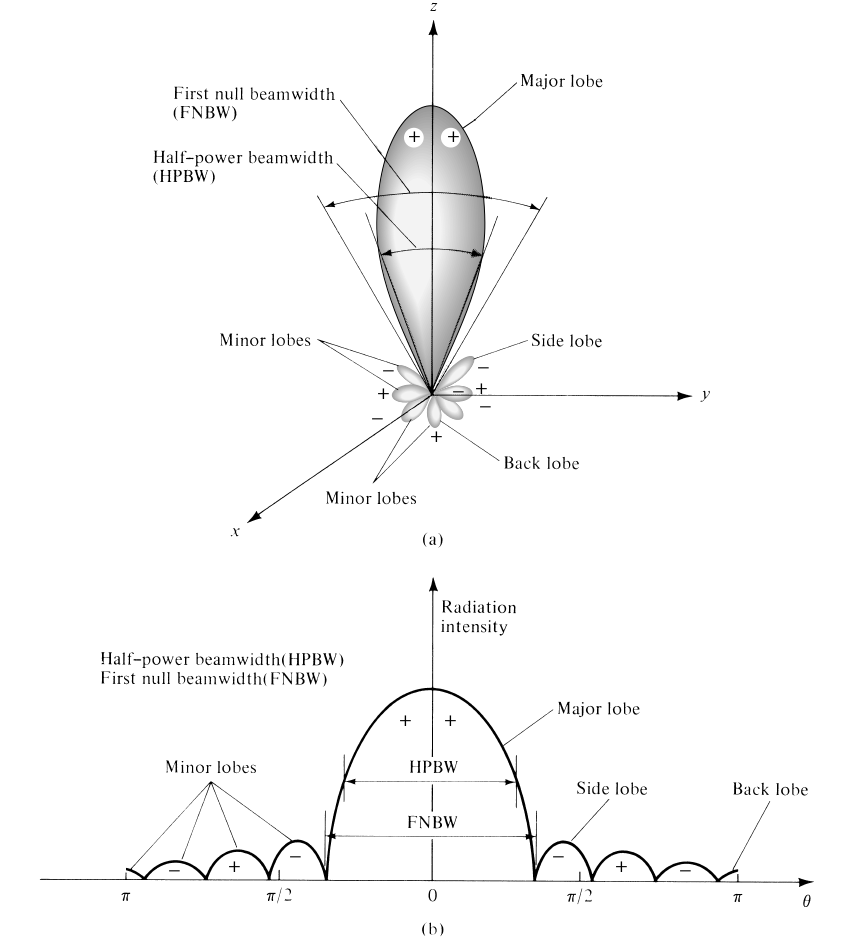
\includegraphics[width=10cm, height=12cm]{c2/radiation-pattern}
% 	    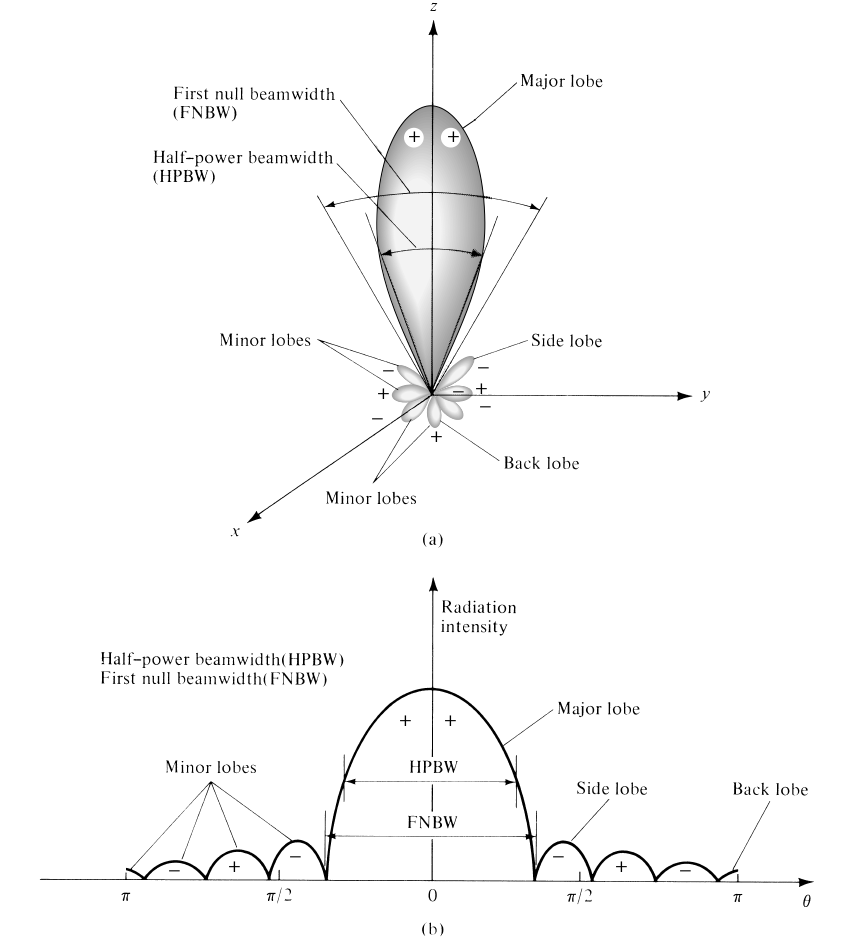
\includegraphics[width=\linewidth]{c2/radiation-pattern}	   	   
	    \caption{(a) Antenna radiation pattern showing the various lobes in angular scales.  (b) Linear projection of the pattern in (a).
	            \emph{Source}: Obtained from \citep[pg. 30]{Balanis2005}}
	    \label{fig:radiation-pattern}
       \end{figure}
  \FloatBarrier   
%%
The portion of the radiation in which the power is accommodated by the antenna is known as \emph{lobes}. We can observe from Fig.~\ref{fig:radiation-pattern} that in one
direction there is maximum power radiation and other directions there are less power radiation. The maximum power radiated in whatever direction is giving us a big lobe
of radiation known as the  \emph{major lobe}. The lobes other than the major lobe are termed  \emph{minor lobes}. These minor lobes are partitioned into \emph{side lobes} 
and \emph{back lobe}. In addition, there are certain directions where radiation drops to zero. The adjacent directions to the major lobe where the radiation drops zero
are known as \emph{null} directions. The null direction close to the major lobe is called the \emph{first null}.
%%

Depending on the shape of the radiation pattern in free space, we have different kinds, namely:
 \begin{itemize}
  \item \emph{Isotropic radiation pattern}:- As the name suggests, between halves there is equal power radiation in all directions. This type of pattern is practically not realistic 
  but the ideal case.
  \item \emph{Directional radiation pattern}:- Fig.~\ref{fig:radiation-pattern} is a typical example of directional antennas such as Cassegrain and Offset Gregorian dishes. 
  Here, we have the maximum radiation  in one direction and zero or less radiation in the other directions.
   \item \emph{Omni-directional radiation pattern}:- It is when the radiation is not in one direction but in equal orthogonal planes.
 \end{itemize}

%%
\subsection{Radiation Intensity}	   \label{chap2:RadiationIntensity}
%% 
This is the power flow per unit solid angle. It can be expressed as;
\begin{equation} \label{eq:rad_intensity}
   \Phi_{\rm rad} = r^{2}\Psi_{\rm rad}    %\frac{r^2}{2\eta}|\bm{E}(r, \theta, \phi)|^2 %   
 \end{equation} 
%  %
 where, $ \Phi_{\rm rad}$ is the radiation intensity  in $\rm Wsr^{-1}$, $\Psi_{\rm rad}$ is the intensity of the electric-field in $\rm Wm^{-2}$ and
 $r $ is the radius of the electric field component.

\subsection{Gain}	   \label{chap2:gain}
%%
The gain of an antenna is the maximum intensity in one direction to the intensity provided by the antenna if the power is radiated uniformly. Mathematically, we can define
this as;

\begin{equation}  \label{eq:gain}
   G = 4\pi\frac{ \Phi_{\rm rad}(\theta, \phi)}{P_{\rm in}}\, \mbox{(dimensionless)}    
 \end{equation} 
 %
where, $\Phi_{\rm rad}(\theta, \phi)$ is the radiation intensity in the direction $(\theta, \phi)$ and $P_{\rm in}$ is the overall accepted power. 

 
 \section{EM Wave Polarization}	   \label{chap2:WavePolarisation}
 %%
 Consider a target source emits an EM wave such that this wave is said to be unpolarized, that is, the electric field of this wave oscillates in every possible position in a plane that is perpendicular to the direction of propagation in the positive $z$ as displayed in Fig.~\ref{fig:emwave}. From Fig.~\ref{fig:emwave}, if the unpolarized wave passes through the polarizing element M1, then M1 will discard all the horizontal components and choose the components in its preferred direction. As a result, the wave that comes out is going to be polarized in the same phase as M1. 
%  a vertical polarizing element 
 %
\begin{figure}[ht]
	    \centering	    
	    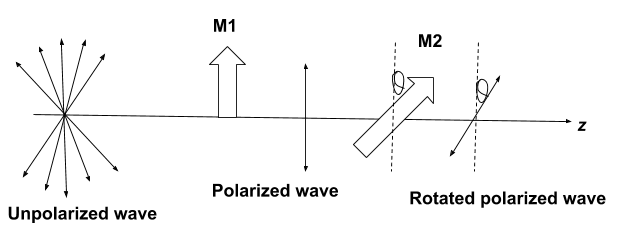
\includegraphics[width=4.2in]{c2/emwave}
	    %\vspace{5 mm}	   
	    \caption{The diagram shows how a polarizing element can polarize an unpolarized wave and also rotate the direction of incoming polarized wave.}
	    \label{fig:emwave}
       \end{figure}
  \FloatBarrier 
%%
 Note that, a polarizing element does not only polarized wave but can also rotate the wave. For instance, if the polarized wave in Fig.~\ref{fig:emwave} goes through
 the polarizer M2  at an angle $\theta$ with respect to the vertical, then M2 ignores all the wave components that are not along the preferred direction  and accepts those along
 angle $\theta$. Therefore, the output wave will still be polarized but rotated at an angle $\theta$. If $\theta = 90^\circ$, then M2 will have horizontal direction that it prefers
 by getting rid of all the vertical parts of the incoming wave. Hence, if M1 is vertical and M2 is horizontal, there would not be any wave that goes through M2.
 
 In Fig.~\ref{fig:emwave}, if we let the electric field $\vec{\xi}$, to be  polarized vertically and propagating in the direction $z$, then the magnetic field $\vec{\mathcal{B}}$ 
 is polarized horizontally (perpendicularly). Here, $\vec{\xi}$  and $\vec{\mathcal{B}}$ conform with the wave equation such that 
 the $\vec{\xi}$ units in the $(x,y)$ coordinates  of a plane-wave can be defined  as Equation~\ref{eq:wav_defn}:
 %%
\begin{subequations}
\begin{align}
\xi_{\rm x}(z, t) & =\, \xi_{\rm 1}\, \cos\{\omega t - \beta z + \varphi_{\rm x} \} \label{eq:wav_defna} \\
\xi_{\rm y}(z, t)  & =\, \xi_{\rm 2}\, \cos\{\omega t - \beta z + \varphi_{\rm y} \} \label{eq:wav_defnb}
%\phantom{\hspace{1cm}}  
 \end{align} 
 \label{eq:wav_defn}
\end{subequations}
%
%
\noindent where, the constant terms $\xi_{\rm 1}$ and $\xi_{\rm 2}$ characterise the maximum amplitude of $(x, y)$ components respectively, 
the radial frequency is $\omega = 2\pi \nu$, the ellipticity measure is expressed as $\beta = 2 \pi / \lambda$ 
and $\varphi_{\rm x}, \varphi_{\rm y}$ are phases of $\xi_{\rm x}$ and $\xi_{\rm y}$ respectively.
Equations~\ref{eq:wav_defna} and \ref{eq:wav_defnb} represent the two linearly polarized waves in the horizontal and vertical orientations respectively. Rewriting
Equation~\ref{eq:wav_defn} vectorially, we get Equation~\ref{eq:add_wav}:
%% Q5
\begin{subequations}
\begin{align}  
   \bm{\xi}(z, t)  & =\, \bm{\hat{x}}\xi_{\rm x}(z, t) + \bm{\hat{y}}\xi_{\rm y}(z, t)\\
		& =\, \bm{\hat{x}}\xi_{\rm 1}\, cos\{\omega t - \beta z + \varphi_{\rm x} \} + \bm{\hat{y}}\xi_{\rm 2}\, cos\{\omega t - \beta z + \varphi_{\rm y} \}   
 \end{align} 
 \label{eq:add_wav}
\end{subequations} 
 % 
 where, $\bm{\hat{x}},\bm{\hat{y}} = $ unit vectors in $x$ and $y$ directions. Therefore, at $z = 0$, Equation~\ref{eq:add_wav} becomes:
 
 
 %% Q6
\begin{equation}  
   \bm{\xi}(t)  = \bm{\hat{x}}\xi_{\rm 1}\, cos\{\omega t + \varphi_{\rm x} \} + \bm{\hat{y}}\xi_{\rm 2}\, cos\{\omega t + \varphi_{\rm y} \}  
  \label{eq:at_z}
 \end{equation} 
 % 
 
\noindent As clearly presented in \cite{Kraus1966}, by eliminating the time $t$ in Equation~\ref{eq:at_z}, we obtain the most general expression of an ellipse as
given in Equation~\ref{eq:gen_wav}:
%% Q7
\begin{equation}  
   a\xi_{\rm x}^2 - b\xi_{\rm x}\xi_{\rm y} + c\xi_{\rm y}^2  = 1  
  \label{eq:gen_wav}
 \end{equation} 
 
\noindent where, $a = 1/\xi_{\rm 1}^2\, \sin^{2}(\varphi)$, $b = 2\, \cos(\varphi)/\xi_{\rm 1}\xi_{\rm 2}\, \sin^{2}(\varphi)$, $c = 1/\xi_{\rm 2}^2\, \sin^{2}(\varphi)$ 
and $\varphi = \varphi_{\rm y} - \varphi_{\rm x}$.

Equation~\ref{eq:gen_wav} shows that at any specific time $t$, the locus of points characterised by the propagation of $\xi_{\rm x}$ and $\xi_{\rm y}$ will trace out this curve. In 
Equation~\ref{eq:gen_wav}, the product term $\xi_{\rm x}\xi_{\rm y}$ actually shows a rotated ellipse. Obviously,  if $\xi_{\rm 1} = 0$,  Equation~\ref{eq:add_wav} becomes linearly 
polarized in the vertical orientation, and vice versa if $\xi_{\rm 2} = 0$. When $\varphi = +90$ and $\xi_{\rm 1} = \xi_{\rm 2}$,
a \textit{left circularly polarized} wave is produced and  when $\varphi = -90$, it is known to be \textit{right circularly polarized}.


 % -------------------------------------------------------------------------------------------------------------------------------------

\subsection{Derivation of the Stokes Polarization Parameters}	   \label{chap2:sec3.1}
%
Section~\ref{chap2:WavePolarisation} dealt with fully polarized waves where, $\xi_{\rm 1},\xi_{\rm 2}$ and $\varphi$ are considered constants. 
A monochromatic (i.e. single-frequency) radiation is of that form. However, generally, in radio observation, the emission from astronomical objects expands
across a multi-frequency range and the bandwidth $\Delta \nu$, consists of incoherently polarized waves due to the superposition of independent waves of different polarizations.
In this section, we present a review of the formulation of Stokes parameters discussed by \cite{Kraus1966}. If we assume two plane waves are orthogonal and let $z = 0$ in Equation~\ref{eq:wav_defn}, 
we get  Equation~\ref{eq:plane_wav}:
% consider a pair of plane waves that are orthogonal to each other at a point in space and choosing  :
%% Q8
\begin{subequations}
\begin{align}
\xi_{x}(t) & =\, \xi_{\rm 1}(t)\, \cos\{\omega t  + \varphi_{\rm x} (t) \} \label{eq:plane_wava} \\
\xi_{y}(t)  & =\, \xi_{\rm 2}(t)\, \cos\{\omega t + \varphi_{\rm y}(t) \} \label{eq:plane_wavb}
%\phantom{\hspace{1cm}}  
  \end{align}
  \label{eq:plane_wav}
\end{subequations}
%
The time variations of $\xi_{\rm 1}(t),  \xi_{\rm 2}(t), \varphi_{\rm x} (t)$ and $\varphi_{\rm y} (t)$ are very slow compared to that of the mean frequency, 
$\nu \,(\omega = 2\pi \nu)$ which is of the order of the bandwidth $\Delta \nu$. Eliminating $\omega t $ term explicitly between Equations~\ref{eq:plane_wava} and \ref{eq:plane_wavb}
we get a similar expression in Equation~\ref{eq:gen_wav}:
%
%% Q9
\begin{equation}
  \begin{aligned}
   \frac{\xi_{\rm x}^2(t)}{\xi_{\rm 1}^{2}(t)} - 2 \frac{\xi_{\rm x}(t)\xi_{\rm y}(t)}{\xi_{1}(t)\xi_{2}(t)}\cos\, \varphi(t)  + \frac{\xi_{\rm y}^2(t)}{\xi_{2}^{2}(t)}  = \sin^{2}\, \varphi (t)
  \end{aligned}
%    \phantom{\hspace{1cm}}
  \label{eq:similar}
 \end{equation} 
%
where, $\varphi(t) = \varphi_{\rm y}(t) - \varphi_{\rm x}(t)$. Equation~\ref{eq:similar} reduces into Equation~\ref{eq:gen_wav} when monochromatic radiation is considered,
making $\xi_{\rm x}$ and $\xi_{\rm y}$ implicitly time dependent.

In order to measure the intensity of a radio wave, we compute the average per the time of observation and  assume the time taken to be infinite because 
it takes a lot time to oscillate per cycle. The time average for Equation~\ref{eq:similar} is therefore represented as:
%
%% Q10
\begin{equation}
  \begin{aligned}
   \frac{\langle \xi_{\rm x}^{2}(t)\rangle}{\xi_{\rm 1}^{2}} - 2 \frac{\langle \xi_{\rm x}(t)\xi_{\rm y}(t)\rangle}{\xi_{\rm 1}\xi_{\rm 2}}\cos\, \varphi  +
   \frac{\langle \xi_{\rm y}^{2}(t)\rangle}{\xi_{\rm 2}^{2}}  = \sin^{2}\, \varphi 
   \end{aligned}
%    \phantom{\hspace{1cm}}
  \label{eq:time_avg}
 \end{equation} 
%
where the symbol $\langle \, \rangle$ denotes the time average and 
%
%% Q11
\begin{equation}
  \begin{aligned}
   \langle \xi_{\rm i}(t)\xi_{\rm j}(t)\rangle = \lim_{T \to \infty} \int\limits_0^T \, \xi_{\rm i}(t)\xi_{\rm j}(t) dt, \quad i, j = x, y
  \end{aligned}
%    \phantom{\hspace{1cm}}
  \label{eq:avg_wav}
 \end{equation} 
%
% 
Multiply Equation~\ref{eq:time_avg} by $4\xi_{\rm 1}^{2}\xi_{\rm 2}^{2}$  and then use Equation~\ref{eq:avg_wav} to compute the average terms in Equation~\ref{eq:time_avg} to get:

%% Q14 
\begin{equation}
  \begin{aligned}
   2\xi_{\rm 1}^{2}\xi_{\rm 2}^{2} - (2\xi_{\rm 1}\xi_{\rm 2}\, \cos\, \varphi )^2 + 2\xi_{\rm 1}^{2}\xi_{\rm 2}^{2} = (2\xi_{\rm 1}\xi_{\rm 2}\, \sin\, \varphi )^2
  \end{aligned}
%    \phantom{\hspace{1cm}}
  \label{eq:wavq}
 \end{equation} 
% %
Representing Equation~\ref{eq:wavq} in perfect square form, we add and subtract $\xi_{1}^{4} + \xi_{2}^{4}$ to get:
%% Q15
\begin{equation}
  \begin{aligned}
   (\xi_{\rm 1}^{2} + \xi_{\rm 2}^{2})^2 - (2\xi_{\rm 1}\xi_{\rm 2}\, \cos\, \varphi )^2 - (\xi_{\rm 1}^{2} - \xi_{\rm 2}^{2})^2 = (2\xi_{\rm 1}\xi_{\rm 2}\, \sin\, \varphi )^2
  \end{aligned}
%    \phantom{\hspace{1cm}}
  \label{eq:deduce}
 \end{equation} 
% %
We can deduce the intensities from Equation~\ref{eq:deduce}:
%% Q16
\begin{subequations}\label{eq:stok}
\begin{align}
P_{\rm I}  & =\,  \xi_{\rm 1}^{2} + \xi_{\rm 2}^{2}	 	\label{eq:stoka} \\
P_{\rm Q} & =\,  \xi_{\rm 1}^{2} - \xi_{\rm 2}^{2} 		\label{eq:stokb} \\
P_{\rm U}  & =\,  2\xi_{\rm 1}\xi_{\rm 2}\, \cos\, \varphi 		\label{eq:stokc} \\ 
P_{\rm V}  & =\,  2\xi_{\rm 1}\xi_{\rm 2}\, \sin\, \varphi  	\label{eq:stokd} 
%\phantom{\hspace{1cm}}
\end{align}
\end{subequations}
%

% \noindent Equation~\ref{eq:stok} is then expressed as:
% % % Q17
% \begin{equation}
%   \begin{aligned}
%    I^2 = Q^2 \, + \, U^2 \, + \, V^2
%   \end{aligned}
% %    \phantom{\hspace{1cm}}
%   \label{eq:intensity}
%  \end{equation} 
%  
\noindent  $I, Q, U\, \textrm{and}\, V$ in Equation~\ref{eq:stok} are the real quantities of Stokes parameters with $I$ being the total intensity. 
 The parameter $Q$ characterises the linear horizontal or vertical polarization; that of $U$ characterises the amount of linear $\pm 45^\circ$ polarization 
 and $V$ represents circular polarization. We can calculate the degree of polarization $P_{\rm {deg}}$, for a given state of polarization:
%% Q18
\begin{equation}
  \begin{aligned}
   P_{\rm deg} = \frac{I_{\rm pol}}{I_{\rm tot}} = \frac{(Q^2 \, + \, U^2 \, + \, V^2)^{1/2}}{I}, \quad 0 \leq P_{\rm deg} \leq 1
  \end{aligned}
   \phantom{\hspace{1cm}}
  \label{eq:q18}
 \end{equation} 
% %
However, ignoring the time average approach and expressing Equations~\ref{eq:plane_wava} and~\ref{eq:plane_wavb} in terms of complex amplitudes to obtain Equation~\ref{eq:q19}:
% \noindent where, $I_{pol}$ is the intensity of the sum of the polarization components and $I_{tot}$ is the total intensity of the signal. $P_{deg} = 1$ 
% relates to completely polarized light, $P_{deg} = 0$ relates to unpolarized light and $0 < P_{deg} < 1$ relates to partially polarized light.
% 
% \noindent The Stokes parameters can also be obtained by ignoring the time average approach and expressing Equations~\ref{eq:plane_wava} and~\ref{eq:plane_wavb} in terms of complex amplitudes:
%% Q19
\begin{subequations}
\begin{align}
\xi_{\rm x}(t) & =\, \xi_{\rm x}\, \exp\{i\omega t \}   \label{eq:q19a} \\
\xi_{\rm y}(t) & =\, \xi_{\rm y}\, \exp\{i\omega t \} 	\label{eq:q19b}
\end{align}
\label{eq:q19}
\end{subequations}
% %
where $\xi_{x} = \xi_{1}\, \exp\{i \varphi_{x} \}$ and $\xi_{y} = \xi_{2}\, \exp\{i \varphi_{y} \}$ are  the complex amplitudes. 
The Stokes polarization parameters from these complex amplitudes are:
% %% Q20
\begin{subequations}
%\begin{eqnarray}
\begin{align}
P_{\rm I}  & =\,  \xi_{\rm x}\xi_{\rm x}^{*} + \xi_{\rm y}\xi_{\rm y}^{*}	 	\label{eq:q20a} \\
P_{\rm Q}  & =\,  \xi_{\rm x}\xi_{\rm x}^{*} - \xi_{\rm y}\xi_{\rm y}^{*}		\label{eq:q20b} \\
P_{\rm U}  & =\, \xi_{x}\xi_{y}^{*} + \xi_{y}\xi_{x}^{*} 		\label{eq:q20c} \\ 
P_{\rm V}  & =\,  i(\xi_{\rm x}\xi_{\rm y}^{*} - \xi_{\rm y}\xi_{\rm x}^{*})		\label{eq:q20d} 
\end{align}
\label{eq:q20}
%\phantom{\hspace{1cm}}  
%\end{eqnarray}
\end{subequations}
% %
% 
These Stokes terms can be used to describe the full polarization state of a signal, for instance, the foregrounds are mostly presented in Stokes parameters.
Chapter~\ref{Chapter4} gives a further detail on how to formulate the Stokes parameters in 
terms of the column matrix to obtain not only measurable intensities but also observables too.
% For a more general discussion on wave polarization see \citep{bkk8,bkk7,bkk9,bkk10,bkk11}. 
% % 
% In short, when an antenna intercepts an EM wave then the polarized instrument depends on the position of observation.
% \noindent Substituting Equations~\ref{eq:q19a} and ~\ref{eq:q19b} into Equation~\ref{eq:q20}, we reproduce the expression in Equation~\ref{eq:q16}. 
% 
% The Stokes parameters give a full characterisation of any polarization state of a plane wave. In Chapter~\ref{Chapter4}, we discuss further on how to formulate the Stokes parameters in
% terms of the column matrix to obtain not only measurable intensities but also observables too. For a more general discussion on wave polarization see \citep{bkk8,bkk7,bkk9,bkk10,bkk11}. 
% 
% In short, an EM wave received by an antenna consists of both electric and magnetic fields. If we are to track the curve traced by the tip of the
% electric field vector, in some fixed location in space, we will get, as time varies, a curve referred to as the polarization ellipse. 
% Also, for a specified location we would generally get different curves, that is to say, the antenna polarization is dependent upon the direction of observation.
%  %
% % -------------------------------------------------------------------------------------------------------------------------------------

 
  \section{Antenna Arrays}	   \label{chap2:sec4}
  %
  Array antenna (also known as interferometer) is the connection of at least two spatially distributed  antennas used to measure or direct the radiation intensity of a source 
  towards a desired angular sector in order to have an improved performance over a single antenna. One unique property of an interferometer is that the beam pattern can be changed when we 
  electronically steer or scan the antenna elements towards some other direction by changing their relative amplitudes and phases. 
  This operation can not be done with a single dish since the beam pattern remains constant. 
%   The use of an array for an observation
%   gives us the opportunity to impose a particular desired array pattern without changing its physical dimensions. Furthermore, by manipulating the received signals from the individual antenna elements in different ways, we can achieve many signal processing
% functions, such as spatial filtering \citep{2009arXiv0910.2865A,2000astro.ph..8239L,2008ISTSP...2..613W}, interference suppression 
% \citep{2008ISTSP...2..670B,2010arXiv1008.5066L,2005RaSc...40.5S11M}, gain enhancement \citep{2008arXiv0809.0208Y}, 
% target tracking \citep{2015PASA...32...17W,2015A&A...573A..99D}, etc.
% %%

% -------------------------------------------------------------------------------------------------------------------------------------

%  (\theta,\phi) = (\vartheta,\varphi)
%
\subsection{Mathematical Formulation of Antenna Array}	    \label{chap2:sec4.1}
%
\theo{
Consider $N$ antenna elements with corresponding radiated electric field $\bar{E}_{k}(\theta,\phi)\mid_{k = 1, 2,3, \ldots, N}$ such that the
angle of elevation and azimuth of these elements are defined  within the range of $-90^{\circ} \leq \theta \leq 90^{\circ}$
and $-180^{\circ}  \leq \phi  \leq 180^{\circ}$ respectively. Then, the overall electric field $\bar{E}(\theta,\phi)$ can be expressed as:
% % Q21
\begin{equation}
  \begin{aligned}
   \bar{E}(\theta,\phi) = \sum_{n = 1}^{N} \, w_{n} \bar{E}_{n}(\theta,\phi)\exp \{i\xi \psi_{n}(\theta,\phi) \}
  \end{aligned}
%    \phantom{\hspace{1cm}}
  \label{eq:q21}
 \end{equation} 
%
where, the element location is $\psi_{n} = x_{n}\sin\, \theta \cos \, \phi + y_{n}\sin\, \theta \sin \, \phi + z_{n}\cos \, \theta $, $\xi = \frac{2\pi}{\lambda}$ is the wavenumber,
$w_{n}|_{n = 1, 2, 3, \ldots, N}$ are the elements complex weights. If the antenna elements are identical, Equation~\ref{eq:q21} becomes;
%
%% Q22
\begin{equation}
  \begin{aligned}
   \bar{E}(\theta,\phi) = \bar{E}_{1}(\theta,\phi)\, \sum_{n = 1}^{N} \, w_{n} \exp \{i\xi \psi_{n}(\theta,\phi) \}
  \end{aligned}
%    \phantom{\hspace{1cm}}
  \label{eq:q22}
 \end{equation} 
%
where $\bar{E}_{1}(\theta,\phi)$ is the element factor and $ \sum_{n = 1}^{N} \, w_{n} \exp \{i\xi \psi_{n}(\theta,\phi) \}$ is the array factor (AF). Equation~\ref{eq:q22}
characterises the \textit{array pattern multiplication}. Assuming we place $N$ antenna elements uniformly linear on a particular 
axis with uniform spacing $n\Delta|_{n = 0, 1, 2, 3,\ldots, N - 1 }$, then:
%
%% Q23
\begin{equation}
  \begin{aligned}
   AF = \sum_{n = 0}^{N-1} \, w_{n} \exp \{i\xi n\Delta \cos\, \theta \}
  \end{aligned}
%    \phantom{\hspace{1cm}}
  \label{eq:q23}
 \end{equation} 
%
where $w_{n} = \exp \{-i\xi n\Delta \, \cos \, \theta_0 \}$. Hence, substituting this into  Equation~\ref{eq:q23}, we get:
%%
%
\begin{equation}
  \begin{aligned}
   AF = \sum_{n = 0}^{N-1} \, (\exp \{i\gamma\})^n, \quad \gamma = \xi\Delta(\cos \theta - \cos \theta_{0})
  \end{aligned}
%    \phantom{\hspace{1cm}}
  \label{eq:af23}
 \end{equation} 
%%
%
% (\exp \{i\gamma\})^n$. letting $\gamma = \xi\Delta(\cos \theta - \cos \theta_{0})$, 
%
\noindent From the geometrical progression theory, we can recall that: 
$$ \sum_{n = 0}^{\infty}\alpha^n = \frac{1}{1 - \alpha}, \alpha \neq 1 \, \mathrm{and} \, \sum_{n = 0}^{N - 1}\alpha^n = \frac{1 - \alpha^N}{1 - \alpha}, \alpha \neq 1$$.
%%
\noindent Applying these two theories to Equation~\ref{eq:af23}, we obtain Equation~\ref{eq:q24}:
% Q24
\begin{subequations}\label{eq:q24}
 \begin{align}
   AF & =\, \frac{1 \, - \, \exp \{ iN\gamma\}}{1 \, - \, \exp \{ i\gamma\}}	\label{eq:q24a}\\ 
     & =\, \frac{\exp \{ iN\gamma/ 2\}}{\exp \{ i\gamma/ 2\}}\frac{\exp \{ iN\gamma/ 2\} - \exp \{ -iN\gamma/ 2\}}{\exp \{ i\gamma/ 2\}-\exp \{ -i\gamma/ 2\}}	\label{eq:q24b}\\ 
      & =\,  \exp \{ i(N - 1)\gamma / 2\}\,\frac{\sin \, (N\gamma/2)}{\sin \, (\gamma/2)} 	\label{eq:q24c}
%        & =\, \exp \{i(N -1)\xi\, \Delta/2 ( \cos\, \theta -  \cos\, \theta_0) \}\,\frac{\sin \, \{ \xi N (\Delta/2)( \cos\, \theta -  \cos\, \theta_0) \}}{
%        \sin \, \{ \xi (\Delta/2)( \cos\, \theta -  \cos\, \theta_0) \}} \label{eq:q24d}
 \end{align}  
 \end{subequations}
%
%
\noindent Since $\sin(Nx)/\sin(x)$ behaves like $N\sinc(x)$, ignoring the phase factor produces Equation~\ref{eq:q26}:
%
%
% %% Q25
% \begin{equation}
%   \begin{aligned}
%    AF = \frac{1}{N} \,  \frac{\sin \, \{ \xi N (\Delta/2)( \cos\, \theta -  \cos\, \theta_0) \}}{
%        \sin \, \{ \xi (\Delta/2)( \cos\, \theta -  \cos\, \theta_0)\}}
%   \end{aligned}
%    \phantom{\hspace{1cm}}
%   \label{eq:q26}
%  \end{equation} 
% %
%
% Q25
\begin{equation}
  \begin{aligned}
   AF = N\sinc  \gamma/2
  \end{aligned}
%    \phantom{\hspace{1cm}}
  \label{eq:q26}
 \end{equation} 
 %
 %
% 
\noindent Therefore, the maximum value of Equation~\ref{eq:q26} occurs when $\gamma = 0$, making $AF = N$. 
% -------------------------------------------------------------------------------------------------------------------------------------
}  % @@@@@@@@@@@@@@@@@@@@@@@@@@@

%
\subsection{Beam-forming}	  	\label{chap2:Beam-forming}
%

The combination of multiple signals with different complex weights from different receiving antenna elements forms a new radiation pattern.
This technique is known as \textit{beam-forming} and can be done in analogue components such as LOFAR with high-band antennas (HBA)
or after the signal is digitised, such as in the LOFAR stations. The algorithms used to generate the technique can be classified into \textit{coherent},
\textit{incoherent} and \textit{multi-pixel beam-former} methods. The application of coherent beam-forming allows a narrow beam to be formed and, 
therefore provides a higher gain which is very useful, for example, during pulsar observation.  Coherent beam-forming increases the sensitivity in narrow FoV.
Unlike coherent beam-forming, incoherent beam-forming does not affect FoV but increases the overall sensitivity. This kind of algorithm is very useful 
when searching for rare events where the location of occurrence is not known. The application of a multi-pixel beam-former like the 
\enquote{Giant Metre wave Radio Telescope} (GMRT\footnote{\url{ http://gmrt.ncra.tifr.res.in/}}) integrates the 
sensitivity of the other two methods by using a \enquote{recorded base-band data} \citep{2012MNRAS.427L..90R} where there is a direct receiving of raw voltage samples 
from the interferometer into an array of storage disks. The technique used for observing pulsars mostly in extended sources can be made more efficiently, 
using the multi-pixel beam-former approach as shown in \cite{deng2017observing}.


% % -------------------------------------------------------------------------------------------------------------------------------------
% 
% %
\subsection{Types of Radio Arrays}	  \label{chap2:sec4.3}
%
In this subsection, we discuss the main types of antenna receiving elements that can be used for radio interferometric observations. The advantages and disadvantages are also
discussed.
%
% -------------------------------------------------------------------------------------------------------------------------------------

\subsubsection{Phased-Array Feeds (PAFs)}	   \label{chap2:sec4.3.1}
%
Generally, a single dish has one pixel and only records the total power captured within its primary beam at any given time. We can produce an image by pointing the single
beam at different directions and then project the output on a sky grid. PAF is a feed design of an antenna dish that consists of elements at reflector focus. 
It is mainly made up of antennas, hardware for signal processing and amplifiers.
% A feed design for a dish, which incorporates multiple feeds instead of the single \enquote{pixel} feed, is referred to as a \enquote{Phased-Array Feed} (PAF). 
This new technology in radio astronomy is the same as having several arrays pointing at different places simultaneously. Its feed
horn is electrically large and collects nearly all focused signal energy. Imaging with an array of multi-beam antennas gives a good resolution and increase in FoV. 
This increase in FoV comes at a cost of each receiving element requiring its own isolated analogue front-end and digital back-end, making the feed more expensive.
This is a new technology undergoing development and currently, PAFs have a higher system temperature and more limited analogue bandwidth than a feed with single pixel.
Even though calibration and how to handle the big data of these new instruments are some of the challenges, their design and ongoing state of development serve as a pathfinder for the SKA \citep{6051207}. 
Some of the PAF-based arrays are the \enquote{Aperture Tile In Focus} (APERTIF\footnote{\url{https://www.astron.nl/astronomy-group/apertif/apertif}}) \citep{oosterloo2009apertif} 
which is an upgrade on  \enquote{Westerbork Synthesis Radio Telescope} (WSRT) and 
\enquote{Australian Square Kilometre Array Pathfinder} (ASKAP\footnote{\url{ http://www.atnf.csiro.au/projects/askap/index.html}}) \citep{johnston2009science}
as displayed in Fig.~\ref{fig:pafs}.
%%
%	+++++++++++++++++++++++++++++++++++++++++++
%	PAFs
%	++++++++++++++++++++++++++++++++++++++++++++
%
\begin{figure}[ht]
	    \centering	    
	    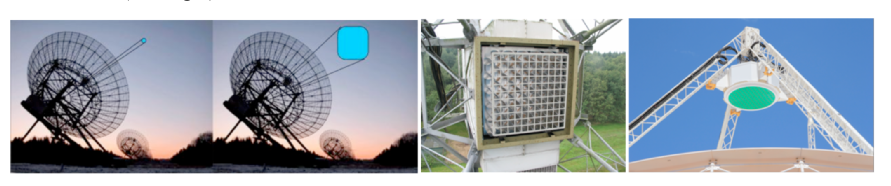
\includegraphics[width=5.8in]{c2/wsrt}
	    %\vspace{5 mm}	   
	    \caption{PAFs showing the wide gain in the FoV. The third image from the left is the installation of APERTIF on WSRT. 
	    The last image from the left displays the PAFs fixed on ASKAP.  \emph{Source}: Reproduced from \cite{garrett2013radio}.
	    }
	    \label{fig:pafs}
       \end{figure}
  \FloatBarrier 
  %
% -------------------------------------------------------------------------------------------------------------------------------------

%
\subsubsection{Transiting Arrays}	   \label{chap2:sec4.3.2}
%
Unlike a dish that can track a particular point in the sky over many hours, a transiting array has elements with limited mobility and allows the sky
to drift through the primary beam of the elements. Its feed has an effective primary beam which is large compared to that of a dish.
As a source enters into the beam, it starts with a small apparent flux, then gradually increases until the source peaks at the zenith. It then decreases as it moves 
across the beam side lobes until it finally sets at the horizon. Some of the  transiting arrays are \enquote{Precision Array for Probing the Epoch of Reionization} (PAPER)
\citep{parsons2010precision},  \enquote{Long Wavelength Array} (LWA) \citep{ellingson2013design}, Medicina Northern Cross and 
the \enquote{Murchison Widefield Array} (MWA\footnote{\url{ http://www.mwatelescope.org/}}) \citep{2009IEEEP..97.1497L} as shown in Fig.~\ref{fig:paper}. Note that
some of the transit arrays such as CHIME, Tianlai, HIRAX, and UTMOST\footnote{\url{https://astronomy.swin.edu.au/research/utmost/}} use collecting elements.
There are obvious cost advantages to building an array with no moving parts. Such arrays have wide FoV and can have the individual elements
placed close together. This allows for large-scale structure experiments, such as Epoch of Reionization (EoR) and BAO studies. 
The disadvantages compared to dishes create a new challenge for calibration and imaging. The individual elements are less sensitive compared to a dish, so more
elements are needed, which requires larger correlator systems. In addition, as the sky transits, the apparent flux of sources changes, so the primary beam must be well known in order 
to get back to the intrinsic flux of the sky. Depending on the scale of the primary beam, a transiting array has a set amount of time per day in which a
section of the sky can be observed. This means that a deep integration of a region of sky is not possible without observing it for many days.
%
%
%	+++++++++++++++++++++++++++++++++++++++++++
%	Transiting Arrays
%	++++++++++++++++++++++++++++++++++++++++++++
%
\begin{figure}[ht]
\centering	    
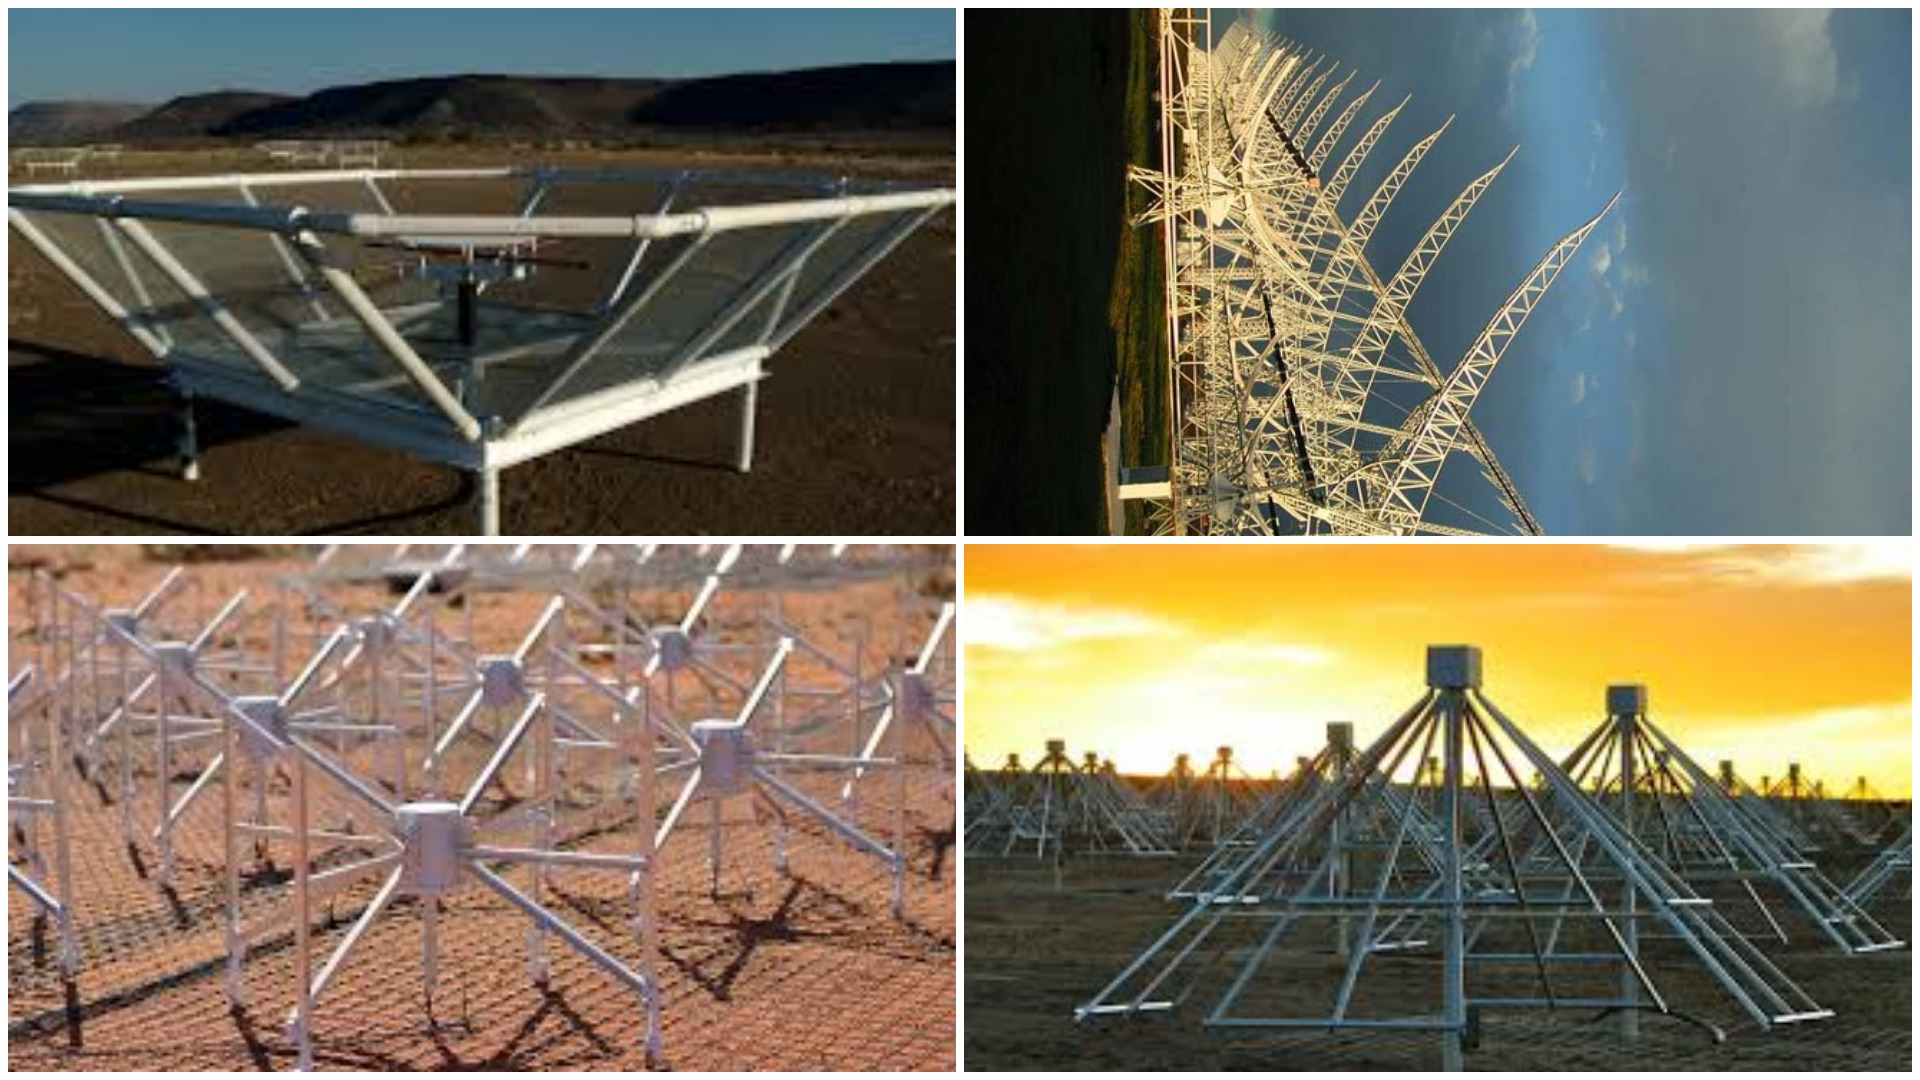
\includegraphics[width=5.8in]{c2/paper-lwa-mwa-cross}
%\vspace{5 mm}	   
\caption{Transiting Arrays:- PAPER (top-left), LWA (bottom-left),  Medicina Northern Cross(top-right) and MWA (bottom-right).}
\label{fig:paper}
\end{figure}
  \FloatBarrier 
  %
  
  % -------------------------------------------------------------------------------------------------------------------------------------

  
\subsubsection{Aperture Arrays}	   \label{chap2:sec4.3.3}
%
We can convert a transiting array into a digital dish to form an \textit{aperture array}. This makes it possible to point the digital dish in many directions of the sky 
simultaneously. The idea with an aperture array is that by updating the beamforming weights, the beam of the aperture array can track a region of the sky. The aperture array takes
advantages from both dishes and transiting arrays. The main cost is the analogue and digital electronics to build such an array. For this reason, aperture arrays are 
mainly used for low-frequency science, such as LOFAR as in Fig.~\ref{fig:lofar} and the future SKA-LOW shown in Fig.~\ref{fig:daa}, as the Dense Aperture Array (DAA) 
components are cheaper. With improved technology, the price of higher frequency components will make it possible to increase the observable frequency. A second issue with aperture arrays is that the primary beam changes, depending on pointing location 
and frequency. As the beam is a weighted sum of all the individual elements there is limited precision to the beam shape. There is a design difference of sparse 
and dense aperture arrays. When the elements of the aperture array are placed closer than $\lambda/2$ observing wavelength the array is \textit{dense}. The array is
fully sampling the wavefront and there are no beam artefacts, such as \textit{grating lobes} (a type of side lobe) which introduces significant structure into the beam. 
If the elements are further apart than $\lambda/2$ then these side lobes structures appear and limit the sensitivity and FoV. For a single observing frequency,
designing an aperture array is simple as all the elements are spaced at $\lambda/2$. However, for wide-band arrays, if the elements are placed at $\lambda_{i}/2$
for a wavelength $\lambda_{i}$ , then for any wavelength $< \lambda_{i}$ the array configuration under-samples that observing wavelength and introduces large grating lobes. 
Therefore, a balance between observing bandwidth, cost and dense versus sparse trade-off must be made during the array design.



%	+++++++++++++++++++++++++++++++++++++++++++
%	Aperture Arrays
%	++++++++++++++++++++++++++++++++++++++++++++
%
\begin{figure}[ht]
    \centering	    
    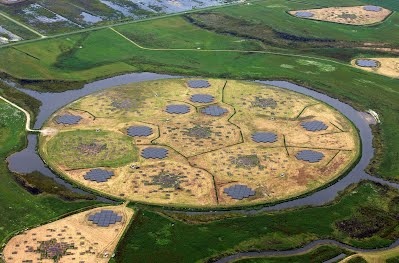
\includegraphics[width=4.2in]{c2/lofar}
    %\vspace{5 mm}	   
    \caption{Aperture Array:- LOFAR.}
    \label{fig:lofar}
\end{figure}
  \FloatBarrier 
  %
%
%	+++++++++++++++++++++++++++++++++++++++++++
%	future Aperture Array
%	++++++++++++++++++++++++++++++++++++++++++++
%
\begin{figure}[ht]
    \centering	    
    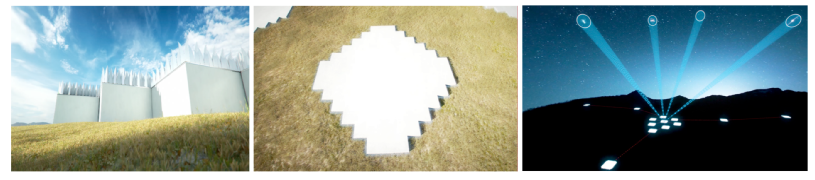
\includegraphics[width=5.8in]{c2/DAA}
    %\vspace{5 mm}	   
    \caption{SKA-2 Dense Aperture Arrays precursor telescope.}
    \label{fig:daa}
\end{figure}
  \FloatBarrier 
%   %
A more detailed discussion on radio arrays can be seen in \cite{techreport-minimal3}.
%

  % -------------------------------------------------------------------------------------------------------------------------------------
 
  \section{Power gained from Radio Sources}	   \label{chap2:sec5a0}
  
The receivers of a radio telescope are very sensitive to the orientation state of the incoming radiation. More generally, in radio astronomy, two receivers are 
attached to each receiving feedhorn, with a splitter feeding horizontally polarized radiation to one receiver
and vertically polarized radiation to the other. The sum of what is obtained in each polarization is known as the \emph{total intensity}. In each polarization, 
the power $P_{w}$ received per unit bandwidth from an element of solid angle of the sky is defined as Equation~\ref{eq:pwr};
%%
\begin{equation} \label{eq:pwr}
P_{w} = \frac{1}{2}A_{e}\iint\limits_{\varOmega}\, B_{s}(\theta,\phi)P_{n}(\theta,\phi)\, d\varOmega 
\end{equation}

\noindent where $A_{e} = $ effective aperture (collecting area) of antenna $\mathrm{[m^{-2}]}$,\\
$B_{s}(\theta,\phi) = $ brightness distribution of radio emission across the sky $\mathrm{[Wm^{-2}Hz^{-1}sr^{-1}]}$,\\
$P_{n}(\theta,\phi) =$ normalised power (beam) pattern of the antenna,\\
$d\varOmega = \sin\theta\, d\theta d\phi$, element of solid angle $\mathrm{[sr]}$.
%%

 In radio astronomy, what we are mostly interested in is the integral of the brightness over a radio source say $S$. The notation $S$ defined in Equation~\ref{eq:flx}
 is the \emph{flux density}: 
%%
\begin{equation} \label{eq:flx}
 S = \iint\limits_{source} \, B_{s}(\theta,\phi) \, d\varOmega
\end{equation}
%%

\noindent Consider the radio source is observed with a radio telescope with the power pattern $P_{n}(\theta, \phi)$, then, 
the observed flux density is computed by the product of the integral of the brightness distribution and the antenna beam pattern:

%%
\begin{equation} \label{eq:flxa}
 S_{0} = \iint\limits_{source} \, B_{s}(\theta,\phi)P_{n}(\theta,\phi) \, d\varOmega
\end{equation}
%%

\noindent In Equation~\ref{eq:flxa}, if we have a radio point source at the phase centre of the beam, then, $P_{n}(\theta,\phi)\simeq 1$ and $S \simeq S_0$, but if the 
source is extended with simple geometry, then simple analytic function will enable $S_0$ to be corrected and this is discussed in the \cite{Gaylard2012} technical report. 
The SI unit of flux density is usually expressed in $\mathrm{Wm^{-2}Hz^{-1}}$. Nevertheless, the radio emission is not very strong because it is emitted from a distant radio source,
and the unit is mostly expressed as Jansky [Jy] which is named after the radio astronomer Karl Jansky. Here,  $1 \mathrm{Jy} \equiv \mathrm{10^{-26} Wm^{-2}Hz^{-1}}$.


%  \section{Brightness Temperature and Antenna Temperature}	   \label{chap2:sec5a}
%  
%  Radio astronomy can be seen as a blend of astronomy and the fundamental of electric circuit theory. Therefore, a
%  radio telescope can be considered as an electric circuit and the source being observed
% can be taken as a resistor at a specific temperature connected to the first amplifier in the receiver
% (by radio waves rather than by wires). For some astronomical sources, the temperature that is determined can be 
% meaningful as a physical temperature or not, depending on the radiation mechanism involved,
% and we therefore, refer to the \emph{brightness temperature} $T_{B}$ for these emitters. For instance, the gas producing the emission may have a physical temperature of  $< 200$ K, but
% the very intense stimulated emission of the maser could have a $T_{B}$ of $1012$ K. $T_{B}$ can be related to the Rayleigh-Jeans law:
% %%
% \begin{equation} \label{eq:ray}
%  T_{B} = \frac{\lambda^{2}}{2k_{B}\varOmega}S \,\mathrm{[WHz^{-1}]}
% \end{equation}
% 
% where $\lambda$ the wavelength, $k_{B}$ the Boltzmann constant, $\varOmega$ the beam solid angle and $S$ the flux density of a source, all in mks units.  
% For a Gaussian beam, its solid angle $\varOmega$  is related to the HPBW $\theta$ by:
% %%
% \begin{equation} \label{eq:omega}
%  \varOmega = \frac{\pi\theta^2}{4\ln 2} %\mathrm{[radians]}
% \end{equation}
% 
% If we observe the radiation from a discrete source which has an effective temperature $T_{B}$ and subtends a solid
% angle $\varOmega$, the source flux density is simply the product of the brightness and the source solid
% angle:
% 
% \begin{equation} \label{eq:src}
%  S = \frac{2k_{B}T_{B}\varOmega}{\lambda^{2}}\, \mathrm{[Wm^{-2}Hz^{-1}]}
% \end{equation}
% %%
% 
% More generally, if the temperature distribution over the emitter is not uniform, the flux density becomes the integral of the temperature distribution over the object:
% \begin{equation} \label{eq:gsrc}
%  S = \frac{2k_{B}}{\lambda^{2}}\iint\limits_{source} T_{B}(\theta, \phi)\, d\varOmega\, \mathrm{[Wm^{-2}Hz^{-1}]}
% \end{equation}

 
  \section{Basic Concepts of Radio Interferometry}	   \label{chap2:Interferometry}
  %
  
  Radio Interferometry is the process of using at least two radio elements to observe astronomical sources. When we synthesize the signals
  from the array along with the electronics we term it the interferometer. For a single telescope, the angular resolution is approximated as 
  $\theta_R \simeq \rm wavelength \, of \, the \,signal (\lambda) / \rm  dish\, diameter (D)$. 
  This means for a particular $\lambda$, if we are interested in a better resolution, then we need to build a telescope with a very large diameter. This is practically tedious and very expensive. Meanwhile, for an interferometer, it modifies $D$ to 
  the longest baseline $\lvert \vec{B} \rvert$. This separation accesses the effective diameter of the array. So, it is more cost effective and realistic to build an interferometer than a very large single dish.
  Therefore, a real-time interferometer for a flat-sky (that is, narrow field of view) is a set of complex visibilities defined in 2D Fourier transform as presented in
  Equation~\ref{eq:vis} :
  %%
  \begin{equation} \label{eq:vis}
 \Lambda_{\rm ab}^{vis}(u, v) = \iint\, A_{\rm ab}^{beam}(\gamma_1,  \gamma_2)I_{\rm ab}^{sky}(\gamma_1,  \gamma_2)\exp[-2\pi j (u\gamma_1 + v\gamma_2)] d\gamma_1 d \gamma_2       %\frac{2k_{B}T_{B}\varOmega}{\lambda^{2}}\, \mathrm{[Wm^{-2}Hz^{-1}]}
\end{equation}
%%
where;
\begin{itemize}
 \item $(u,v)$ denote the coordinates of a pair of antennas $a,b$ in the $uv-$plane. These coordinates are related to the baseline
 per unit wavelength such that $(u,v, 0) \propto \vec{B}/\lambda$, $u$ is the east-west line of $\vec{B}$, and $v$ is the north-south line of $\vec{B}$. Note that
 since we assume the visibility sampling is measured on a plane, our field of view becomes narrow and therefore, we ignore the $w-$term such that $w = 0$. 
%  This  If our visibility sampling is approximately on a plane, or again we are only interested in a narrow field of view then the so-called w-term
 \item $(\gamma_1,  \gamma_2)$ are the direction cosine in the image plane and so, they are related to the source position $\hat{\mathbf{\varsigma}}$, in the sky such that 
 $(\gamma_1,  \gamma_2, 0) \propto \hat{\mathbf{\varsigma}}$. Here,  $\gamma_1$ is the east-west orientation of $\hat{\mathbf{\varsigma}}$, and $\gamma_2$ 
 is the north-south orientation of $\hat{\mathbf{\varsigma}}$.
 \item the primary beam of two elements is described in $ A_{\rm ab}^{beam}$. 
 \item $I_{\rm ab}^{sky}(\gamma_1,  \gamma_2)$ is the distribution of sky brightness.
\end{itemize}
%%
Equation~\ref{eq:vis} is famously known as \textit{van Cittert-Zernike equation} \citep{Thompson2001,1974Thompson,2009Rau}.

In physical observation, the complex visibility $\Lambda_{\rm ab}^{vis}(u, v)$ is not measured everywhere, but only finite in the $uv$ domain.
Let denote this sampling process as $S_{\rm ab}(u, v)$
such that we record zeros if no data is captured. As a result, the true sky $I_{\rm ab}^{sky}(\gamma_1,  \gamma_2)$,  cannot be recovered directly, instead, we obtain the dirty map $I_{\rm ab}^{dirty}(\gamma_1,  \gamma_2)$,
as given in Equation~\ref{eq:dirty}:
%%
%%
  \begin{equation} \label{eq:dirty}
 I_{\rm ab}^{dirty}(\gamma_1,  \gamma_2) =  A_{\rm ab}^{beam}(\gamma_1,  \gamma_2)I_{\rm ab}^{sky}(\gamma_1,  \gamma_2) \otimes B_{ab}(\gamma_1,  \gamma_2)       %\frac{2k_{B}T_{B}\varOmega}{\lambda^{2}}\, \mathrm{[Wm^{-2}Hz^{-1}]}
\end{equation}
 %%
 $B_{ab}(\gamma_1,  \gamma_2)$ in Equation~\ref{eq:dirty}  is the point-spread function (PSF) describing the $uv$ distribution of baselines and can be expressed as Equation~\ref{eq:psf}:
 %%
  \begin{equation} \label{eq:psf}
 B_{ab}(\gamma_1,  \gamma_2) =  \iint\, S_{\rm ab}(u, v)\exp[2\pi j (u\gamma_1 + v\gamma_2)] d\gamma_1 d \gamma_2 
\end{equation}
 %%
 Hence, we can obtain $I_{\rm ab}^{dirty}(\gamma_1,  \gamma_2)$ by applying the convolution theorem, using the operator $\otimes$. Once a dirty image is made,
 we can deconvolve it to produce an estimate of the true sky map.  The CLEAN algorithm, originally introduced by \citep{hogbom1974aperture} and 
 the \enquote{Maximum Entropy Method} (MEM) \citep{carcamo2018multi} are the common methods of deconvolution.
 
% \subsection{Construction of Radio Images}	  \label{chap2:sec5.1}
%%

%   Radio telescopes are used to measure the flux density of an observed radio source by integrating the intensity over the telescope beam. An intensity image 
%   of the observed source is then produced from the data obtained from the radio telescopes. Fig.~\ref{fig:hg10}(a) as in \citep{2010Joardar} displays a single dish radio telescope steering at a distant radio source with parallel rays illuminating the dish aperture. 
%   Consider that the aperture plane is located at the origin of a rectangular coordinate system $(u,v,w)$ with $w$ pointing directly at the source as in Fig.~\ref{fig:hg10}(b) and
%   the $u$ and $v$ axes point east and north in the $(u,v)$ plane normal to the $w$ axis . 
%   Also, in the sky, consider the electric field distribution to be centred on different coordinate system $(\gamma_1,  \gamma_2)$. These $(\gamma_1,  \gamma_2)$ are the direction cosines
%     projected onto the $(u, v)$ plane. The electric field distribution $\varepsilon(u,v)$ on   the $u,v$ plane is defined in terms of the electric field distribution of $V(\gamma_1,  \gamma_2)$ in the sky.
%     Considering that we have all the information regarding $\varepsilon(u,v)$, we can then find the auto-correlation of each of the electric field points on the $u,v$ plane to get $W(u,v)$. 
%     The intensity field distribution $I(\gamma_1,  \gamma_2)$ of the source is measured when we find the Fourier transform on $W(u,v)$. Realistically $\varepsilon(u,v)$ is not achievable,
%     since the antenna produces a single output. This single output is very significant as it shows a basic relation between intensity map of radio source in the sky with the aperture 
%     illumination.
% %
% %
% %	+++++++++++++++++++++++++++++++++++++++++++
% %	Measure Image
% %	++++++++++++++++++++++++++++++++++++++++++++
% %
% \begin{figure}[ht]
% 	    \centering	    
% 	    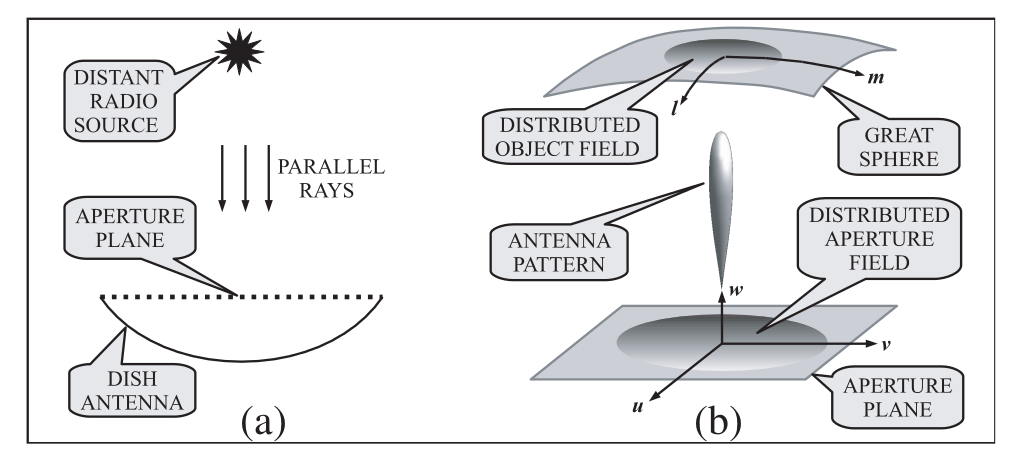
\includegraphics[width=4.2in]{c2/measure-image}
% 	    %\vspace{5 mm}	   
% 	    \caption{(a) \textit{A distant radio astronomical source illuminates a dish antenna with parallel rays.}
% 	    (b) \textit{Electric field distributions of a source on the great sphere and antenna aperture on the aperture plane}}
% 	    \label{fig:hg10}
%        \end{figure}
%   \FloatBarrier 
%   %
%   \noindent  Although single dish radio telescopes, such as the $100$ m GBT and the huge but fixed $305$ m Arecibo Observatory are very advantageous
%     in making primary surveys of the sky at low resolution, the resolution of a telescope is limited by its collecting area  \citep{wright2004single,2002Emerson}.
%     Interferometry is a technique for connecting multiple radio antennas to efficiently form single antenna with a far greater collecting area than the individual components.
%     The separation between the antennas and the rotation of the Earth leads to differences in the observed path length from the object under observation.
%     When the data from each of the antennas is put together, an interference pattern is generated, which can be reconstructed to form an image of the observation.
%     %     However, its data can be put together with antenna array also known as interferometer to obtain a good balance between lower and higher spatial frequency components.\\    
%  Instead of a single dish antenna, an interferometer with the assistance of the rotation of Earth can synthesise a large antenna aperture. This technique is known as 
%  \textit{super-synthesis} \citep{1952Machin,1974Thompson}.
%  
%  Consider a large number of radio telescopes distributed across a plane area situated at a given longitude, latitude and altitude as shown in Fig.~\ref{fig:hg11}(a), 
%  such that they track a distant radio source located on the celestial North pole. Consider also a rectangular coordinate system $(u',v',w')$ whose origin is
%  at the phase centre of telescope plane as in Fig.~\ref{fig:hg11}(b), reproduced from \citep{2010Joardar}, such that $w'$ axis points towards the zenith (source) 
%  and the $u',v'$ plane remains stationary to the observed source. From the observed source towards the antennas, due to the rotation of the Earth, 
%  the position of the antennas appears to be moving over the  $u',v'$ plane.  The outputs of individual radio telescopes is recorded at each integration time and then placed on the $u',v'$ plane.
% %
% %	+++++++++++++++++++++++++++++++++++++++++++
% %	Aperture synthesis
% %	++++++++++++++++++++++++++++++++++++++++++++
% %
% \begin{figure}[ht]
% 	    \centering	    
% 	    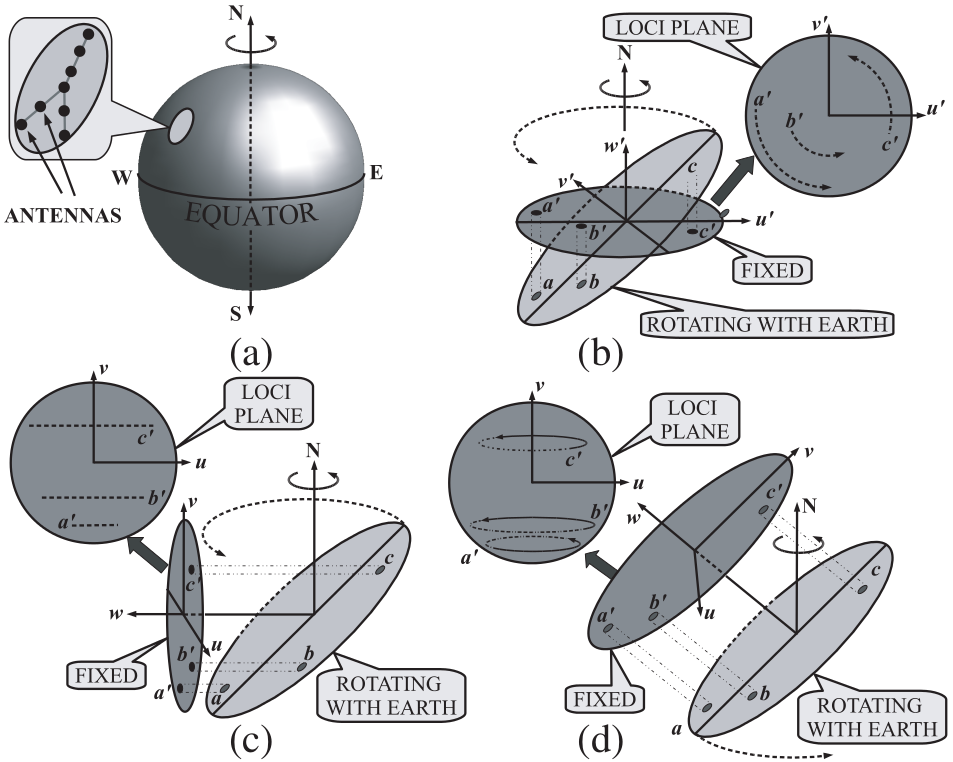
\includegraphics[width=4.2in]{c2/super-synthesis}
% 	    %\vspace{5 mm}	   
% 	    \caption{\textit{The principle of super synthesis}. (a) \textit{An interferometer rotates with the Earth rotation}
% 	    (b) \textit{Observing a radio source towards celestial North Pole.} 
% 	    (c) \textit{Observing a radio source along the celestial equator.}
% 	    (d) \textit{Observing a radio source along a celestial latitude in between.}}
% 	    \label{fig:hg11}
%        \end{figure}
%   \FloatBarrier 
%   %
%  The loci $a' , b'$ and $c'$ of the radio telescopes $a, b$ and $c$ respectively on the $u',v'$ plane forms circles over a period of 24 h.  Having numerous radio telescopes at 
%  different baselines from the origin of the $(u' , v' , w')$ coordinates over a period of 24 h,  the $u',v'$ plane gets highly populated. The $u ',v'$ plane then forms the
%  aperture of a large synthesised antenna. Thus, we apply Fourier transform on the $u',v'$ plane data after calibration to obtain the field distribution of the source.
% %
% Considering a radio source on the celestial equator as presented in Fig.~\ref{fig:hg11}(c), the loci $a',b'$ and $c'$ on the $u',v'$ plane form straight lines. Thus,
% if all the radio telescopes are mounted on a single East-West line then their respective  loci be a  straight line and this not good enough for making a radio image. It is therefore
% necessary to mount some of the radio telescopes spread along the North-South axis. If the observed source is located at a celestial latitude between $(0^{\circ}, 90^ {\circ})$ or 
% $(-90^{\circ}, 0^ {\circ})$, each of the loci form an ellipse as shown in  Fig.~\ref{fig:hg11}(d).
% %
% %
% \subsection{Correlator Super-Synthesis Arrays}	  	 \label{chap2:sec5.2}
% %
% The correlation products between any pair of antennas are used to fill the $u,v$ plane, where the $(u, v, w)$ coordinates are measured in wavelengths. If there are $N$ antennas 
% in an array, then the number of cross correlation is defined as $N\left(\frac{N-1}{2}\right)$. In any pair of antennas in an interferometer, when we fix one of the antennas 
% at the origin of the $(u, v, w)$, the baseline between the two antennas on the $u,v$ plane will rotate through $180^\circ$ in 12 h. We obtain similar observation results when the 
% other antenna is considered as the origin of the $(u, v, w)$ coordinates. This makes it possible to cover $360^\circ$ of baseline rotation in half a day. Thus, 
% data obtained from an interferometer is a measure of the spatial coherence function called \textit{visibility} and is denoted as $V(u, v)$. This visibility data covers only $1/2$
% of the $u,v$ plane from a 12 h observation, but the other $1/2$ can be obtained using Equation~\ref{eq:q26}, where $V^{*}(u, v)$ is the complex conjugate of
% $V(u, v)$. Hence, we can derive 24 h of observed data from a 12 h observation.
% %% Q26
% \begin{equation}
%   \begin{aligned}
%   V(-u, -v) = V^{*}(u, v)
%    \end{aligned}
%    \phantom{\hspace{1cm}}
%   \label{eq:q26}
%  \end{equation} 
%  %
%  %
%  
% % -------------------------------------------------------------------------------------------------------------------------------------
% 
% \subsection{The Van Cittert-Zernike equation}	  	\label{chap2:sec5.3}
% %
% Consider a two-element interferometer observing a radio source as in  Fig.~\ref{fig:hg12}(a) \citep{2010Joardar} such that the first element is positioned at the origin of the $(u, v, w)$
% coordinate system. In addition, consider $I(\gamma_1,  \gamma_2)$ to be the intensity distribution of the source on the celestial sphere such that the origin of the $l, m$
% coordinate system is at the phase reference position. If we denote $I(\bar{s})$ as the sky brightness at a frequency $\nu$ in the direction $\bar{s}$ and assume 
% $A(\bar{s})$ to be the effective aperture area of an antenna in the same direction, then the signal power received over a bandwidth $\Delta \nu$ within
% a solid angular element $d\Omega$ for each antenna is given by $A(\bar{s}) I(\bar{s}) \Delta \nu d\Omega \cos (2\pi \nu \tau_g)$. Therefore, the  correlated signal power $dr$ over
% $d\Omega$ is given as:
% %% Q27
% \begin{equation}
%   \begin{aligned}
%   dr = A(\bar{s}) I(\bar{s}) \Delta \nu d\Omega \cos (2\pi \nu \tau_g)
%    \end{aligned}
%    \phantom{\hspace{1cm}}
%   \label{eq:q27}
%  \end{equation} 
%  %
%  Integrating Equation~\ref{eq:q27} over the celestial sphere we get the correlator power $r$:
%  %% Q28
% \begin{equation}
%   \begin{aligned}
%   r(\overrightarrow{d}_{\lambda}, \bar{s}) = \Delta \nu \int A(\bar{s}) I(\bar{s}) \cos [2\pi (\overrightarrow{d}_{\lambda} \bar{s})] d\Omega 
%    \end{aligned}
%    \phantom{\hspace{1cm}}
%   \label{eq:q28}
%  \end{equation} 
%  %
%  where $\overrightarrow{d}_{\lambda}$ is the baseline  vector specified by the $(u,v,w)$ coordinates and measured in wavelengths.
% %
% %	+++++++++++++++++++++++++++++++++++++++++++
% %	interferometer synthesis
% %	++++++++++++++++++++++++++++++++++++++++++++
% %
% \begin{figure}[ht]
% 	    \centering	    
% 	    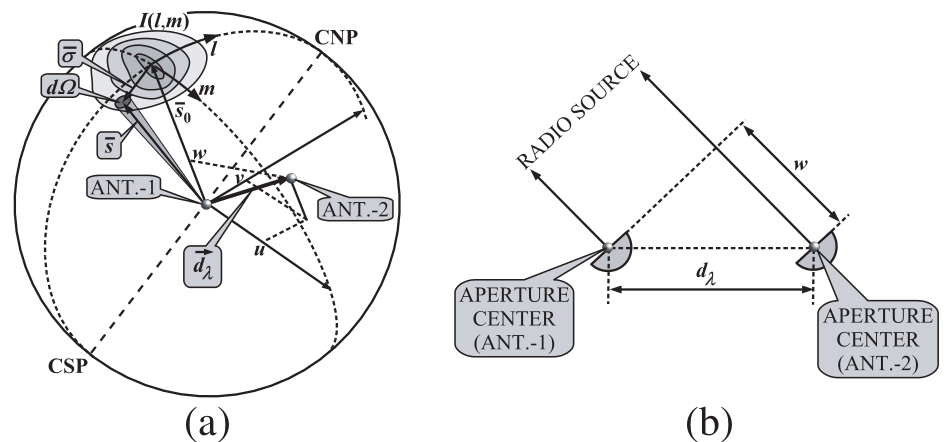
\includegraphics[width=4.8in]{c2/interferometer}
% 	    %\vspace{5 mm}	   
% 	    \caption{\textit{Geometry of a radio source and a simple interferometer}. (a) \textit{An observed radio source with intensity distribution $I(\gamma_1,  \gamma_2)$ 
% 	    using a simple two element radio interferometer.}
% 	    (b) \textit{Lower the elevation angle of the radio source the larger the value of w.} 
% 	    }
% 	    \label{fig:hg12}
%        \end{figure}
%   \FloatBarrier 
%   %
%  \noindent  If we put $ \bar{s} = \bar{\sigma} + \bar{s}_{0}$ such that $\bar{\sigma}$ is the position vector from the phase reference 
%   point to the observing point. Rewriting Equation~\ref{eq:q28} we get:
%    %% Q29
% \begin{equation}
%   \begin{aligned}
%   r(\overrightarrow{d}_{\lambda}, \bar{s}_{0}) = \Delta \nu  \cos [2\pi (\overrightarrow{d}_{\lambda} \bar{s}_{0})]  \int A(\bar{\sigma}) I(\bar{\sigma}) \cos [2\pi (\overrightarrow{d}_{\lambda} \bar{\sigma})] d\Omega\\
% 					-  \Delta \nu  \sin [2\pi (\overrightarrow{d}_{\lambda} \bar{s}_{0})]  \int A(\bar{\sigma}) I(\bar{\sigma}) \sin [2\pi (\overrightarrow{d}_{\lambda} \bar{\sigma})] d\Omega 
%    \end{aligned}
%    \phantom{\hspace{1cm}}
%   \label{eq:q29}
%  \end{equation}  
%  %
%  The visibility $V$ is defined as a complex function:
%   %% Q30
% \begin{equation}
%   \begin{aligned}
%   V = |V| \exp(j\phi_\nu) =  \int A'(\bar{\sigma}) I(\bar{\sigma}) \exp (-j2\pi \overrightarrow{d}_{\lambda} \bar{\sigma}) d\Omega 
%    \end{aligned}
%    \phantom{\hspace{1cm}}
%   \label{eq:q30}
%  \end{equation} 
%  %
%  with the real part being:
%  
%  %% Q31
% \begin{equation}
%   \begin{aligned}
%   V = |V| \cos(\phi_\nu) =  \int A'(\bar{\sigma}) I(\bar{\sigma}) \cos (2\pi \overrightarrow{d}_{\lambda} \bar{\sigma}) d\Omega 
%    \end{aligned}
%    \phantom{\hspace{1cm}}
%   \label{eq:q31}
%  \end{equation} 
%  
%  
%  \noindent and the imaginary part being:
%  
%  %% Q32
% \begin{equation}
%   \begin{aligned}
%   V = |V| \sin(\phi_\nu) =  -\int A'(\bar{\sigma}) I(\bar{\sigma}) \sin (2\pi \overrightarrow{d}_{\lambda} \bar{\sigma}) d\Omega 
%    \end{aligned}
%    \phantom{\hspace{1cm}}
%   \label{eq:q32}
%  \end{equation} 
%  %
% where, $A'(\bar{\sigma}) = \frac{A(\bar{\sigma})}{A_0}$ is the normalised beam pattern of an antenna with $A_0$ being the peak antenna gain.
% Substituting Equation~\ref{eq:q31} into~\ref{eq:q30}, we get:
%  
%   %% Q33
% \begin{equation}
%   \begin{aligned}
%   r(\overrightarrow{d}_{\lambda}, \bar{s}_{0}) = A_{0} \Delta \nu  |V| \cos [2\pi (\overrightarrow{d}_{\lambda} \bar{\sigma} - \phi_\nu)]
%    \end{aligned}
%    \phantom{\hspace{1cm}}
%   \label{eq:q33}
%  \end{equation} 
%  %
%  Equation~\ref{eq:q33} shows that an interferometer measures the visibility which is a measure of the wavefront's spatial coherence across the baseline. 
%  To produce an image from Equation~\ref{eq:q33}, we need to know their positions on the $u, v, w$ coordinate system and compare them with $l, m$ 
%  coordinate system. As the elevation angle of the observed source decreases as in Fig.~\ref{fig:hg12}(b), the $w$ term increases: 
% %% Q34
% \begin{equation}
%   \begin{aligned}
%   \overrightarrow{d}_{\lambda} \bar{s}  = ul + vm + wn
%    \end{aligned}
%    \phantom{\hspace{1cm}}
%   \label{eq:q34}
%  \end{equation} 
%  %
% If $\bar{s} = \bar{s}_{0}$ Equation~\ref{eq:q34} simplifies to:
% %% Q35
% \begin{equation}
%   \begin{aligned}
%   \overrightarrow{d}_{\lambda} \bar{s}  = w
%    \end{aligned}
%    \phantom{\hspace{1cm}}
%   \label{eq:q35}
%  \end{equation} 
%  %
% The solid angle $d\Omega $ can be expressed in polar coordinates as $d\Omega  = \sin \theta\,  d\theta d\phi$, where $\theta$ and $\phi$ are the polar and 
% azimuthal angles in the $(u, v , w)$ plane,that is, $\theta = \sin^{-1} (\sqrt{l^2 + m^2})$ and $\phi = tan^{-1} (m/l)$. Using the Jacobian method, we can transform the 
% coordinates $(\theta, \phi)$ into  $(\gamma_1,  \gamma_2)$:
% %% Q36
% \begin{equation}
%   \begin{aligned}
%   d\Omega = \frac{d\gamma_1 d \gamma_2}{n} = \frac{d\gamma_1 d \gamma_2}{\sqrt{1 - l^2 - m^2}}
%    \end{aligned}
%    \phantom{\hspace{1cm}}
%   \label{eq:q36}
%  \end{equation} 
%  %
% 
% \noindent Using Equations~\ref{eq:q34} to~\ref{eq:q36}, we can therefore rewrite the visibility $V$ in Equation~\ref{eq:q34} in terms of $u, v , w$:
% %% Q37
% \begin{equation}
%   \begin{aligned}
%   V(u,v,w) =  \int\limits_{-\infty}^{\infty} \int\limits_{-\infty}^{\infty} \, \frac{A'(\gamma_1,  \gamma_2) I(\gamma_1,  \gamma_2)}{\sqrt{1 - l^2 - m^2}} \exp \{
%   -j2\pi[ul + vm + w(\sqrt{1 - l^2 - m^2} -1)]\} dl dm
%    \end{aligned}
%    \phantom{\hspace{1cm}}
%   \label{eq:q37}
%  \end{equation} 
%  %
% 
% \noindent Equation~\ref{eq:q37} is known as \textit{van Cittert-Zernike equation} \citep{bkk13,1974Thompson,2009Rau} and it shows that the visibility $V(u, v, w)$, 
% is a Fourier transform of the product of the sky brightness $I(\gamma_1,  \gamma_2)$, the primary beam response $A'(\gamma_1,  \gamma_2)$ and $1/\sqrt{1 - l^2 - m^2}$. 
% When the distance of the observed source becomes less, $|l|$ and $|m|$ become much less such that $w(\sqrt{1 - l^2 - m^2} -1)$ approaches zero and Equation~\ref{eq:q37} reduces to:
% 
% %% Q38
% \begin{equation}
%   \begin{aligned}
%   V(u,v,w) \simeq V(u,v,0) =  \int\limits_{-\infty}^{\infty} \int\limits_{-\infty}^{\infty} \, \frac{A'(\gamma_1,  \gamma_2) I(\gamma_1,  \gamma_2)}{\sqrt{1 - l^2 - m^2}} \exp \{-j2\pi(u\gamma_1 + v\gamma_2)\} dl dm
%    \end{aligned}
%    \phantom{\hspace{1cm}}
%   \label{eq:q38}
%  \end{equation} 
%  %
% and the inverse transform being defined by:
% 
% %% Q39
% \begin{equation}
%   \begin{aligned}
%   \frac{A'(\gamma_1,  \gamma_2) I(\gamma_1,  \gamma_2)}{\sqrt{1 - l^2 - m^2}}  =  \int\limits_{-\infty}^{\infty} \int\limits_{-\infty}^{\infty} \, V(u,v)  \exp \{j2\pi(u\gamma_1 + v\gamma_2)\} du dv 
%    \end{aligned}
%    \phantom{\hspace{1cm}}
%   \label{eq:q39}
%  \end{equation} 
%  %
%  %
%  
%  % -------------------------------------------------------------------------------------------------------------------------------------
% 
% \subsection{Filling the \emph{u,v} Plane with Visibilities}	  \label{chap2:sec5.}
% %
% Consider the phase reference position of an observed radio source is at $(H_{0}, \varphi_{0})$ in the local equatorial coordinate system. Assume $X_{\lambda}, Y_{\lambda}$ and
% $Z_{\lambda}$ are the baseline components in a rectangular coordinate system measured in wavelengths \citep{bkk13}, then the $u,v$ can be written as;
% %% Q40
% \begin{equation}
%   \begin{aligned}
%   u^{2} + \left[\frac{v - Z_{\lambda}\cos(\varphi_{0})}{\sin (\varphi_{0})}\right]^{2} = X_{\lambda}^{2} + Y_{\lambda}^{2}
%    \end{aligned}
%    \phantom{\hspace{1cm}}
%   \label{eq:q40}
%  \end{equation} 
%  %
%  Equation~\ref{eq:q40} represents an ellipse which splits into $2$ in the $u, v$ plane if $Z_{\lambda} \neq 0$  \citep{bkk13}. Fig.~\ref{fig:hg13}(a) produced from \citep{2010Joardar}
%  displays Equation~\ref{eq:q40} when observing a radio source at declination $\varphi_{0})$. That for Fig.~\ref{fig:hg13}(b) displays cases of a North-South baseline for 
%  different values of $\varphi_{0}$.
% %	+++++++++++++++++++++++++++++++++++++++++++
% %	declination plot
% %	++++++++++++++++++++++++++++++++++++++++++++
% %
% \begin{figure}[ht]
% 	    \centering	    
% 	    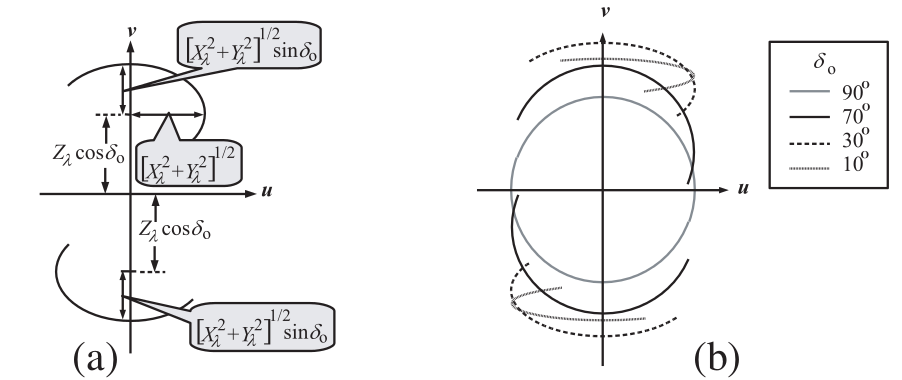
\includegraphics[width=4.8in]{c2/uv-plane}
% 	    %\vspace{5 mm}	   
% 	    \caption{\textit{Locus on the $u, v$ plane.}. (a) \textit{Locus of the
% ellipse on $u, v$ plane for a baseline with $Z_{\lambda} \neq 0$ observing a radio source at declination $\varphi_{0}$.}
% 	    (b) \textit{Different declinations for different cases.} 
% 	    }
% 	    \label{fig:hg13}
%        \end{figure}
%   \FloatBarrier 
%   %
% \noindent The KAT-7 consists of seven observing antennas located at latitude $-30^{\circ}$, longitude $21^{\circ}$ and altitude $1038 \,\mathrm{m}$ in configuration as shown in Fig.~\ref{fig:hg14}(a).
% Fig.~\ref{fig:hg14}(b) displays the $u,v$ coverage at particular synthesis time with observed radio source at the phase centre. The circular structure rotates along with the Earth.
% If the zenith coincides with a celestial pole, then each point traces out a circle. Otherwise, the tracings could be elliptical, broken ellipse, or straight line (zero declination).
% When we increase the synthesis time, more data fill the \emph{uv} plane. Using Equation~\ref{eq:q39}, the intensity distribution $I(\gamma_1,  \gamma_2)$ or image of the radio source is made. This is 
% actually done after calibrating the data \cite{bkk13,1974Thompson,2009Rau,2016arXiv160302126B,2016A&A...586A..76J}.
%  %
%  \begin{figure}[ht]
%   \centering
%      \begin{subfigure}[b]{0.49\textwidth}
%                 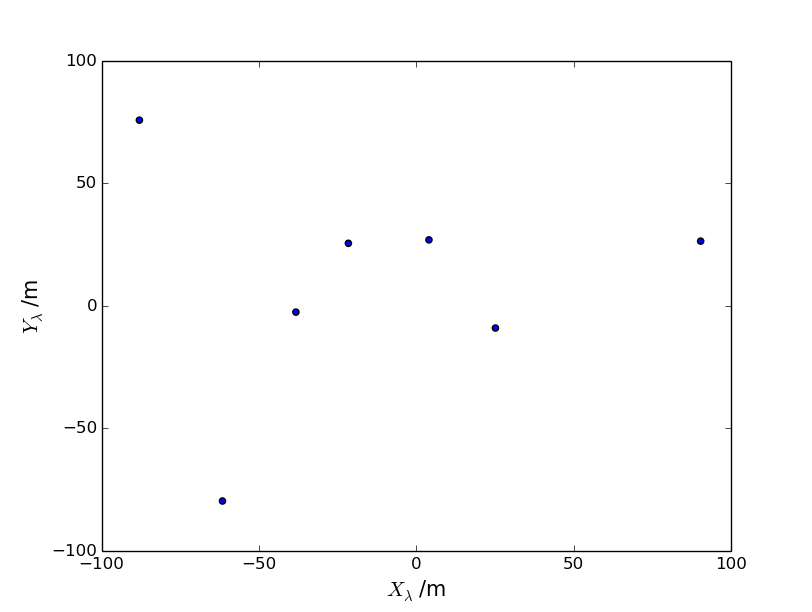
\includegraphics[width=\textwidth]{c2/kat7-setup}
%                 \caption{}
%                 %\label{fig:lab0}
%         \end{subfigure}       
%         \begin{subfigure}[b]{0.50\textwidth}
%                 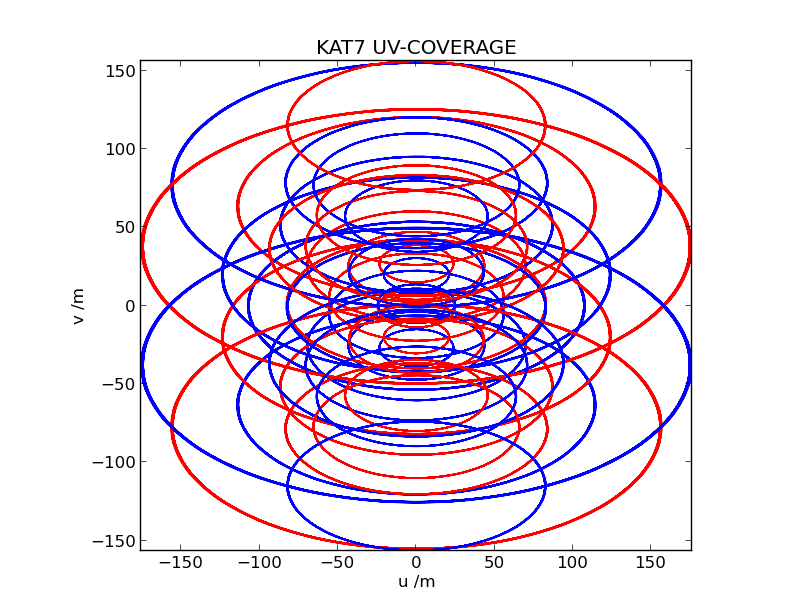
\includegraphics[width=\textwidth]{c2/msuv}
%                 \caption{}
%                % \label{fig:lab1}
%         \end{subfigure}
%         \caption{\textit{Filling the u-v plane with visibilities}. (a) \textit{The KAT-7 configuration.}
% 	    (b) \textit{The u-v plane coverage of a $4 \,\mathrm{h}$ period of observation obtained from a source at the phase centre.} 
% 	    }
% 	    \label{fig:hg14}
%   \end{figure}
% \FloatBarrier 
% %
% 
% \noindent Using the Fast Fourier Transform (FFT) approach, the data on \emph{u,v} plane is interpolated on a uniform grid \citep{bkk13,2005Fu,2007Zhang} and 
% at the same time employs the tapering technique \citep{bkk13} to reduce the side lobes of the synthesised antenna beam. The dirty image obtained after FFT may contain lots of 
% artefacts \citep{2016arXiv160107182D}. These are removed using algorithms such as  CLEAN \citep{2009GGG....10.9U07A,1998Camps,2010ISPM...27...14L,2012JPhCS.355a2020C} or
% MEM \citep{2012JPhCS.355a2020C,2016A&A...586A..76J,2013arXiv1307.6757C}. 







% %	+++++++++++++++++++++++++++++++++++++++++++
% %	kat7 image plot
% %	++++++++++++++++++++++++++++++++++++++++++++
% %
% \begin{figure}[ht]
% 	    \centering	    
% 	    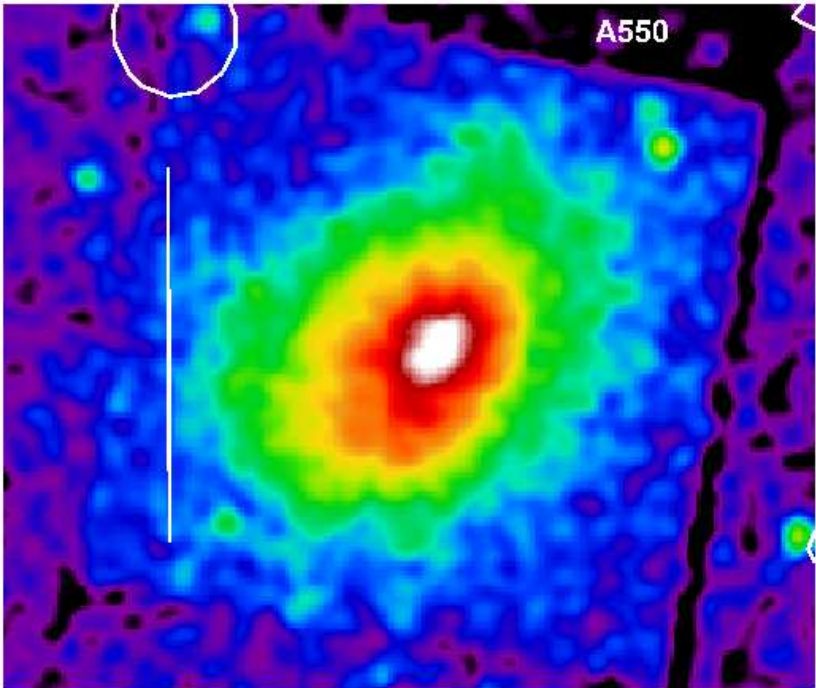
\includegraphics[width=4.8in]{c2/GB}
% 	    %\vspace{5 mm}	   
% 	    \caption{\textit{: 1.86 GHz KAT–7 radio contours of the A 550 cluster overlaid on the X–ray XMM–Newton images as an example of target that does
% 	    not show any diffuse radio emission corresponding to the cluster centre. 
% 	    The image is not corrected by the primary beam. The vertical white bar indicates a $800 kpc$ size.}. 
% 	    }
% 	    \label{fig:hg15}
%        \end{figure}
%   \FloatBarrier 
%   %
% Fig.~\ref{fig:hg15} displays $1.86$ GHz KAT–7 radio contours of the A 550 cluster as in \citep{2016arXiv160307595B} and drawn at $-2.5, 2.5, 10$ and $40 \, mJy\, beam^{-1}$
% with positive (negative) contours drawn using solid (dashed) lines. 
% 
% 
% 
% 

















 
